% \documentclass{article}
\documentclass[12pt,a4paper,oneside,fleqn]{book}
\usepackage[slovene]{babel}
% \usepackage[english]{babel}

% \usepackage[a4paper,top=2cm,bottom=2cm,left=3cm,right=3cm,marginparwidth=1.75cm]{geometry}
\usepackage[left=30mm,
right=25mm,
top=30mm,
bottom=25mm]{geometry}

% \usepackage[backend=biber, style=ieee]{biblatex}
\usepackage{cite}
\usepackage[numbib]{tocbibind}
% \addbibresource{refs.bib}

\usepackage{lipsum}
\usepackage{array}
\usepackage{caption}
\usepackage{amsmath}
\usepackage{graphicx}
\usepackage{subcaption}
\usepackage[colorlinks=true, allcolors=blue]{hyperref}
\usepackage[nodisplayskipstretch]{setspace}
\usepackage{fancyhdr}
\usepackage{listings}
\usepackage{xcolor}

\definecolor{codegreen}{rgb}{0,0.6,0}
\definecolor{codegray}{rgb}{0.5,0.5,0.5}
\definecolor{codepurple}{rgb}{0.58,0,0.82}
\definecolor{backcolour}{rgb}{0.95,0.95,0.92}

\lstdefinestyle{codestyle}{
    backgroundcolor=\color{backcolour},   
    commentstyle=\color{codegreen},
    keywordstyle=\color{magenta},
    numberstyle=\tiny\color{codegray},
    stringstyle=\color{codepurple},
    basicstyle=\ttfamily\footnotesize,
    breakatwhitespace=false,         
    breaklines=true,                 
    captionpos=b,                    
    keepspaces=true,                 
    % numbers=left,   
    numbers=none,
    numbersep=5pt,                  
    showspaces=false,                
    showstringspaces=false,
    showtabs=false,                  
    tabsize=2
}
\renewcommand{\lstlistingname}{Kod}
\lstset{style=codestyle}


%paragraph settings
\setlength\parindent{0pt}
\setlength{\parskip}{1.5ex plus 0.5ex minus 0.5ex}

% set equation environment indentation
\setlength{\mathindent}{0.5cm}%

% set itemize environment whitespacing and left margin
% \setlist[itemize]{noitemsep,nolistsep, leftmargin=*}

% set table and figure captions
\captionsetup[table]{skip=10pt,singlelinecheck=false}
\captionsetup[figure]{justification=centering}

% set tablename to Preglednica
\AtBeginDocument{%
	\renewcommand\tablename{Preglednica}
}

% set section and tableofcontents depth
\setcounter{secnumdepth}{3}
\setcounter{tocdepth}{3}
\def\labelitemi{--}

%  accordingly format a chapter definition
% \titleformat{\chapter}[display]
% {\bfseries}{}{0pt}{\Huge\thechapter\quad}

% set fancy_nohead fancy header
\fancypagestyle{fancy_nohead}{
	\fancyfoot[RO]{\thepage}
	\fancyhead{}
	\renewcommand{\headrulewidth}{0pt}
	\chead{}
	\cfoot{}
}

% assign no_header
% \assignpagestyle{\chapter}{fancy_nohead}

\renewcommand{\thetable}{\arabic{chapter}.\arabic{table}}
\renewcommand{\thefigure}{\arabic{chapter}.\arabic{figure}}
\renewcommand{\theequation}{\arabic{chapter}.\arabic{equation}}

% \renewcommand\cftchapdotsep{\cftdotsep}  % adds leader dots from chapter titles to page numbers

\usepackage[T1]{fontenc} % Ensures proper font rendering
\usepackage{lmodern}  

% \title{OracleDepth Phase1}
\title{Interdisciplinarni projekt: Kamera kalibracija in 3D rekonstrukcija z Meshroom}
\author{Kristijan Danov 23221364}
\date{}

\begin{document}

\maketitle

\tableofcontents
\newpage

\pagenumbering{arabic}
\chapter{Uvod}
    V tem poročilu bomo obravnavali osnovno teorijo modela proste kamere(pinhole), ChArUco markerje in kalibracijo kamere. Uporabili bomo tudi kodo python za izvedbo kalibracije kamere in nepopačenje slik. In izvedli bomo 3D rekonstrukcijo v Meshroom 2023.3.0. Za kodo bomo uporabili Python 3.11 in naslednje module:
\begin{itemize}
    \item numpy==1.24.2
    \item opencv\_contrib\_python==4.11.0.86
\end{itemize}

\chapter{Teorija}
    Da bi razumeli, kaj delamo z našo kodo, moramo najprej imeti dobro teoretično osnovo. Tukaj bomo preučili nekaj osnov o prostih kamerah, parametrih kamer, popačenju, kalibracijah kamer itd.

\section{Pinhole kamera}
    Modela proste kamere(pinhole) je idealiziran matematični opis razmerja med tridimenzionalnim prostorom in dvodimenzionalno projekcijo slike. Pinhole kamera je sestavljena iz majhne odprtine (pinhole) in slikovne ravnine. Ker se odprtina nahaja med slikovno ravnino in 3D svetom, mora vsak žarek, ki izvira iz 3D prostora, preiti skozi odprtino, preden doseže slikovno ravnino. V tem primeru je projicirana slika obrnjena (\ref{fig:obscura}a). Ta naravni pojav se imenuje kamera obskura in je bil uporabljen skozi zgodovino, opisal pa ga je Ibn al-Haytham v 10. stoletju. Če pa pred odprtino postavimo ravnino, projicirana slika ne bo obrnjena (\ref{fig:obscura}b). 

\begin{figure}[h]
    \centering
    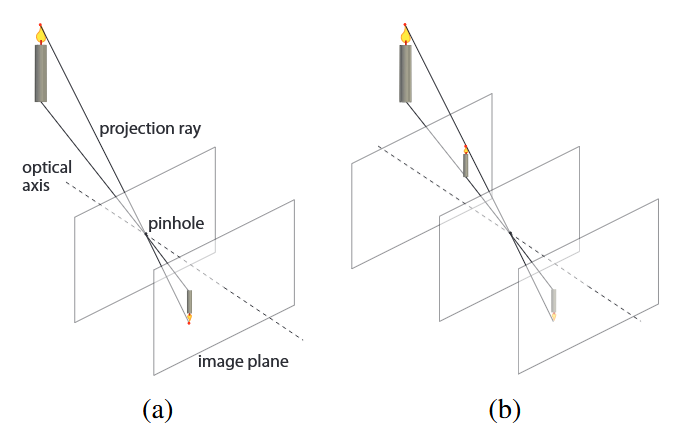
\includegraphics[width=0.5\linewidth]{imgs/obscura.png}
    \caption{Pinhole kamera\cite{Tomasi_2025a}}
    \label{fig:obscura}
\end{figure}

Za matematično razumevanje tega modela moramo najprej definirati 2 pomembna koordinatna sistema\cite{Cyganek_Siebert_2010}. To so:
\begin{itemize}
    \item Zunanji koordinatni sistem('W' za 'world') z izhodišče $\pmb{O_W}$ in osmi $[X_W, Y_W, Z_W]$
    \item Kamera koordinatni sistem('C' za 'camera') z izhodišče $\pmb{O_C}$ in osmi $[X_C, Y_C, Z_C]$
\end{itemize}



\begin{figure}[h]
    \centering
    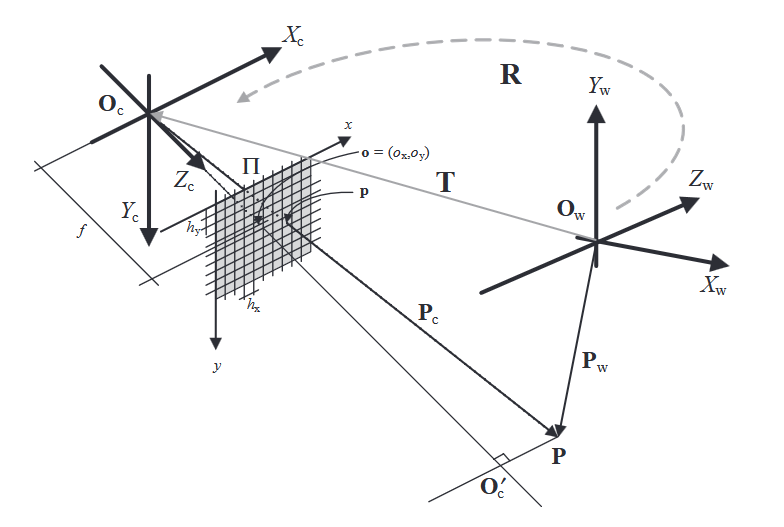
\includegraphics[width=0.8\linewidth]{imgs/pinholemodel.png}
    \caption{Koordinatni sistemi in točke v pinhole kamera\cite{Cyganek_Siebert_2010}}
    \label{fig:pinhole}
\end{figure}

Ta dva koordinatna sistema sta povezana z translacijo $\pmb{t}$ in rotacijo $\pmb{R}$. \\
Naslednje točke lahko vidite na sliki \ref{fig:pinhole}. \\
Slikovna ravnina $\pmb{\Pi}$ je razrezana v pravokotnike, imenovane piksli. Piksli v kameri tvorijo diskretna mesta za zaznavanje fotografije, ki vzorčijo katero koli sliko, projicirano na ravnino. Vsak piksel je indeksiran s parom koordinat, izraženih z naravnimi številkami. $h_x$ in $h_y$ določata fizične dimenzije ene piksle. \\
Točka $\pmb{O_C}$, se imenuje goriščna točka. Njena projekcija na $\pmb{\Pi}$ v smeri $Z_C$ določa glavno točko $o$ na slikovni ravnini. Razdalja od goriščne točke $\pmb{O_C}$ do glavne točke $o$ se imenuje goriščna razdalja $f$. $Z_C$ se imenuje tudi glavna os. Na njej ležijo $\pmb{O_C}$, $o$ in $\pmb{O_C'}$.\\
V realnem svetu lahko določimo neko točko $\pmb{P}$, njen položaj pa je podan z izbranim koordinatnim sistemom, $\pmb{P_C}$ za koordinatni sistem kamere ali $\pmb{P_W}$ za zunanji koordinatni sistem. \\
Točka $\pmb{p}$ je slika točke $\pmb{P}$ na slikovno ravnino s središčem $\pmb{O_C}$. Njihove koordinate lahko definiramo kot:
\[
    \pmb{P} = [X, Y, Z]^T  \qquad \pmb{p} = [x, y, z]^T
\]
Ker imamo podobna trikotnika $\triangle\pmb{O_C p o}$ in $\triangle\pmb{O_C P O_C'}$ dobimo:
\[
    x=f\frac{X}{Z} \qquad y=f\frac{Y}{Z} \qquad z =f
\]
Model pinhole kamere lahko definiramo z dvema skupinama parametrov:
\begin{itemize}
    \item Zunanji parametri(extrinsic)
    \item Notranji parametri(intrinsic)
\end{itemize}

    \subsection{Zunanji parametri}
        Zunanji parametri so vsi geometrijski parametri, potrebni za prehod iz zunanji koordinatni sistem v koordinatnega sistema kamere. Ta prehod je opisan s translacijo $\pmb{t}$ in rotacijo $\pmb{R}$. Spremembo točke $\pmb{P}$, podane v svetovnih koordinatah kot $\pmb{P_W}$, v koordinatni sistem kamere $\pmb{P_C}$ lahko zapišemo kot:
\[
    \pmb{P_C} = \pmb{R}(\pmb{P_W}-\pmb{t})
\]
Zunanji parametri $\pmb{t}$ in $\pmb{R}$ so zapisani kot:
\[
    \pmb{t} = \pmb{O_W} - \pmb{O_C} = \begin{bmatrix}
                                        T_1 \\
                                        T_2 \\
                                        T_3
                                        \end{bmatrix}_{3\times3}
                                        \qquad
    \pmb{R} =
    \begin{bmatrix}
        \pmb{R_{1}} \\
        \pmb{R_{2}} \\
        \pmb{R_{3}} \\
    \end{bmatrix}_{3\times3}
    = \begin{bmatrix}
        R_{11} & R_{12} & R_{13} \\
        R_{21} & R_{22} & R_{23} \\
        R_{31} & R_{32} & R_{33} \\
    \end{bmatrix}_{3\times3}
\]
Zunanje parametre lahko zapišemo kot matriko $\pmb{M_e}$.
\[
    \pmb{M_e} = 
    \begin{bmatrix}
        \pmb{R_1} & -\pmb{R_1 t} \\
        \pmb{R_2} & -\pmb{R_2 t} \\
        \pmb{R_3} & -\pmb{R_3 t} \\        
    \end{bmatrix}_{3\times4}
\]
    
    \subsection{Notranji parametri}
        Notranji parametri so goriščna razdalja $f$ in parametri, ki preslikajo koordinatni sistem kamere na slikovno ravnino (tu so tudi parametri popačenja, vendar jih za zdaj ne bomo upoštevali). \\
Te notranje parametre lahko zapišemo kot matriko $\pmb{M_i}$.\[
    \pmb{M_i} = 
    \begin{bmatrix}
        \frac{f}{h_x} & 0 & o_x \\
        0 & \frac{f}{h_y} & o_y \\
        0 & 0 & 1
    \end{bmatrix}_{3\times3}
\]

\section{Projektivna transformacija}
    Preslikava točke $\pmb{P}$ v $\pmb{p}$ na slikovni ravnini se izvede s transformacijo $\pmb{M}$.
\[
    \pmb{p} = \pmb{M P}
\]
Matrika $\pmb{M}$ se imenuje projekcijska matrika in je sestavljena iz matrik notranjih in zunanjih parametrov.
\[
    \pmb{M} = \pmb{M_i M_e}
\]


\section{Popačenje}
    V resničnem svetu pinhole kamere niso praktične, ker je slika zamegljena, če je odprtina prevelika, in pretemna, če je premajhna. Zato uporabljamo leče, ki vhodne žarke preusmerijo na slikovno ravnino. Zaradi uporabe leč pride do popačenja. Tukaj bomo obravnavali radialno in tangencialno popačenje. \\
Naj bodo $(x, y)$ koordinate točke na nepopačeni sliki in $(x_d, y_d)$ koordinate te iste točke na popačeni sliki. \\
Radialno popačenje povzroča ``barrel" ali ``fish-eye" efekt v slikah. Radialno popačenje lahko predstavimo kot
\begin{gather}
    x_d = x(1 + k_1 r^2 + k_2 r^4 + k_3 r^6) \notag\\
    y_d = y(1 + k_1 r^2 + k_2 r^4 + k_3 r^6) \notag\\
    r^2 = x^2+y^2
    \label{radialdistEq}
\end{gather}
\begin{figure}[h]
    \centering
    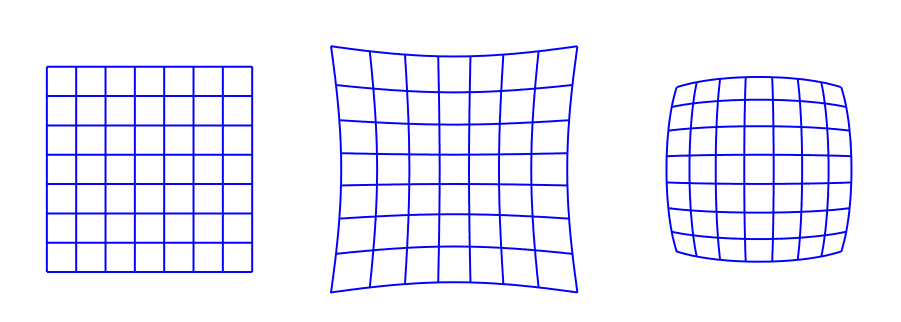
\includegraphics[width=0.5\linewidth]{imgs/radialdist.png}
    \caption{Radialno popačenje\cite{Tomasi_2025a}}
    \label{fig:raddist}
\end{figure}

Tangencialno popačenje nastane, ker leče niso popolnoma vzporedne s slikovno ravnino, in ga lahko predstavimo kot
\begin{gather}
    x_d = x+[2p_1xy+p_2(r^2+2x^2)] \notag\\
    y_d = y+[p_1(r^2+2y^2)+2p_2xy]
    \label{tangentialdistEq}
\end{gather}

Da bi ugotovili koeficiente popačenja $(k_1, k_2, p_1, p_2, p_3)$ ter notranje in zunanje parametre, izvedemo kalibracijo kamere\cite{calibtut}.

\section{Kalibracija kamere}
    Kalibracija kamere je postopek ugotavljanja notranjih, zunanjih parametrov in koeficientov popačenja. Ena od njihovih uporab je odstranjevanje popačenja. \\
Kalibracija temelji na reševanju osnovnih geometrijskih enačb na podlagi izbranega kalibrirnega objekta. Zaznamo vogale vzorca. Najpogostejši so ChArUco vzorci. Vzorci ChArUco so sestavljeni iz šahovnice in ArUco vzorcev. ArUco markerji imajo hitro zaznavanje, vendar njihova natančnost ni visoka. Šahovnice imajo večjo natančnost, ker je vsak vogal obdan z dvema črnima poljema, vendar mora biti popolnoma viden in ga je težje zaznati. S kombinacijo teh dveh dobimo najboljše od obeh. Z ArUco markerji lahko interpoliramo položaje vogalov šahovnice, kar omogoča delne poglede. Tudi zaradi ArUco markerji ima lahko vsak vogal šahovnice unikaten ID, ki ni odvisen od tega, ali je vzorec obrnjen.

\begin{figure}[h]
    \begin{subfigure}{.5\textwidth}
        \centering
        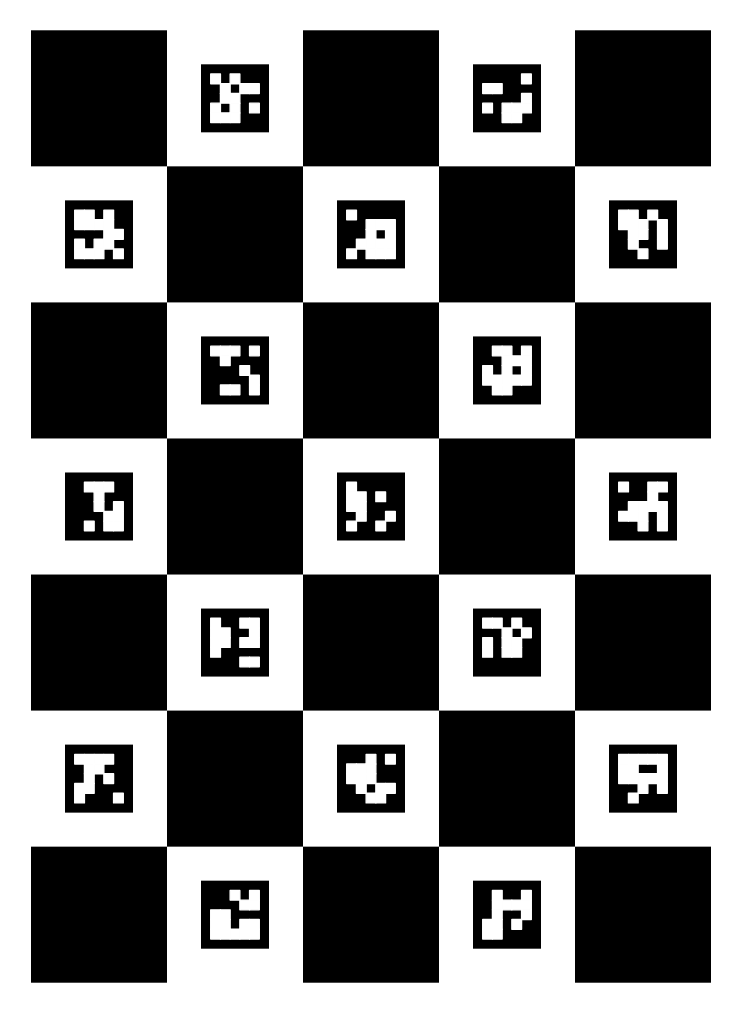
\includegraphics[width=.95\linewidth]{imgs/charuco.png}
        \caption{Primer plošče}
    \end{subfigure}
    \begin{subfigure}{.5\textwidth}
        \centering
        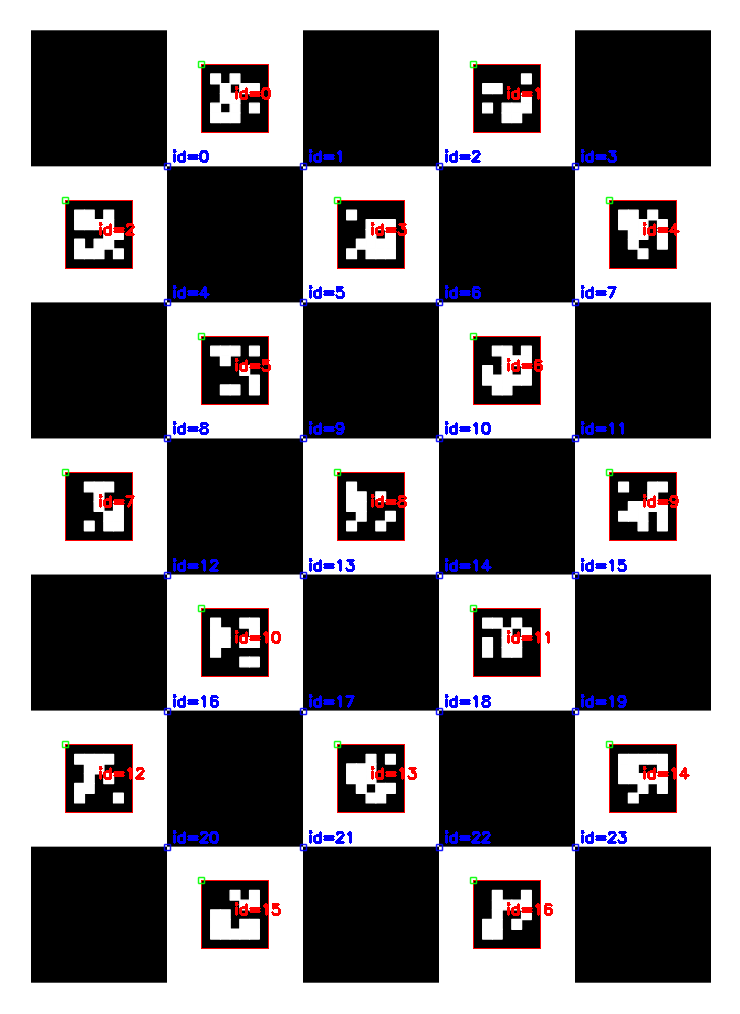
\includegraphics[width=.95\linewidth]{imgs/charucoDetect.png}
        \caption{Plošča z zaznanimi markerji in vrisanimi vogali}
    \end{subfigure}
    \caption{ChArUco plošča}
\end{figure}

\subsection{Zhangova metoda za izračun notranjih parametrov}
V tem pododdelku bomo preučili matematiko v Zhangovi metodi za kalibracija kamere.\cite{zhang}\cite{calibyt}\\

Začnimo s pisanjem enačbe, ki povezuje 3D točko s točko 2D slike. Leva in desna matrika sta notranja in zunanja matrika. Notranja matrika je zapisana nekoliko drugače kot prej, ker tukaj upoštevamo asimetrijo in razmerje stranic(aspect ratio).
\[
    \begin{bmatrix}
    x \\
    y \\
    1 
    \end{bmatrix}
    =
    \begin{bmatrix}
    c   &   cs  &   x_H \\
    0   &   c(1+m)  &   y_H \\
    0   &   0   &   1 
    \end{bmatrix}
    \begin{bmatrix}
    r_{11}   &   r_{12}  &  r_{13}  &   t_1 \\
    r_{21}   &   r_{22}  &  r_{23}  &   t_2 \\
    r_{31}   &   r_{32}  &  r_{33}  &   t_3
    \end{bmatrix}
    \begin{bmatrix}
        X \\
        Y \\
        Z \\
        1
    \end{bmatrix}
\]
S predpostavko, da je $Z=0$ (ko uporabljamo plošče, vse točke na ploščah imajo enako vrednost $Z=0$), lahko odstranimo tretji stolpec zunanja matrike.
\begin{equation}
    \begin{bmatrix}
    x \\
    y \\
    1 
    \end{bmatrix}
    =
    \begin{bmatrix}
    c   &   cs  &   x_H \\
    0   &   c(1+m)  &   y_H \\
    0   &   0   &   1 
    \end{bmatrix}
    \begin{bmatrix}
    r_{11}   &   r_{12}  &   t_1 \\
    r_{21}   &   r_{22}  &   t_2 \\
    r_{31}   &   r_{32}   &   t_3
    \end{bmatrix}
        \begin{bmatrix}
        X \\
        Y \\
        1
    \end{bmatrix}
    \label{simplifiedmappingLong}
\end{equation}
Zelo pomembno je omeniti, da so notranji parametri enaki za vsako sliko (in tako vsako točko na vsaki sliki), medtem ko so zunanji parametri enaki za vsako točko na sliki (spreminjajo se od slike do slike). \\
Transformacijo lahko zapišemo kot 3x3 matriko $H$. Tu je $K$ notranja matrika. Z $H$ lahko zapišemo krajšo obliko \ref{simplifiedmappingLong} za vsako točko $i$, ki je na sliki.
\begin{equation}
H=[\pmb{h_1}, \pmb{h_2}, \pmb{h_3}]=K[\pmb{r_1}, \pmb{r_2}, \pmb{t}]
\label{defH}
\end{equation}
\begin{equation}
    \begin{bmatrix}
        x_i \\
        y_i \\
        1 
    \end{bmatrix}
    =
    H
    \begin{bmatrix}
        X_i \\
        Y_i \\
        1 
    \end{bmatrix}
    \quad
    i=1,...,I
    \label{simMap}
\end{equation}
Od tu naprej, če bi poznali zunanjo matriko, bi lahko samo naredili QR dekompozicijo $H$ in našli naše parametre (Q bi bila zunanja matrika, R bi bila notranja matrika). Vendar ni tako. Najti moramo način z uporabo lastnosti $K$ in zunanje matrike, da izvlečemo $K$ iz $H$. Po tem lahko najdemo zunanje parametre. \\
Začnimo z prepisovanjem enačbe \ref{defH} z inverzijo matrike $K$. Iz te enačbe lahko pridobimo enačbe za $r_1$ in $r_2$.
\begin{gather}
    \begin{bmatrix}
        \pmb{r_1}, \pmb{r_2}, \pmb{t}
    \end{bmatrix}
    =
    K^{-1}
    \begin{bmatrix}
        \pmb{h_1}, \pmb{h_2}, \pmb{h_3}
    \end{bmatrix}   \notag\\
    \notag\\
    \pmb{r_1}=K^{-1}\pmb{h_1} \notag\\
    \pmb{r_2}=K^{-1}\pmb{h_2}
    \label{r1r2}
\end{gather}
Za rotacijske vektorje vemo da so ortogonalni in enotski vektorji. V te enačbe lahko vstavimo enačbe iz \ref{r1r2}. (Opomba: $K^{-T}=(K^{-1})^T$ in $\|\pmb{r_1}\|=\pmb{r_1}^T \pmb{r_1}$)
\begin{gather}
    \pmb{r_1}^T \pmb{r_2}=0 \qquad \Longrightarrow \qquad \pmb{h_1}^TK^{-T}K^{-1}\pmb{h_2}=0    \notag\\
    \|\pmb{r_1}\|=\|\pmb{r_2}\|=1 \qquad \Longrightarrow \qquad \pmb{h_1}^T K^{-T}K^{-1}\pmb{h_1}-\pmb{h_2}^TK^{-T}K^{-1}\pmb{h_2}=0
    \label{hKeqs}
\end{gather}
Definirajmo matriko $B$ in prepišimo \ref{hKeqs}. Ker ima matrika $K$ samo realne vrednosti, je matrika $B$ pozitivno definirana matrika.
\begin{gather}
    B=K^{-T} K^{-1} \label{Bdef} \\
    \pmb{h_1}^T B \pmb{h_2}=0 \notag\\
    \pmb{h_1}^T B \pmb{h_1}-\pmb{h_2}^T B \pmb{h_2}=0
    \label{hBeqs}
\end{gather}
Upoštevajte, da je $B$ matrika, pomnožena z isto transponirano matriko. To matriko lahko najdemo z razcep Choleskega. Z dekompozicijo matrike $B$ bo naš rezultat transponirana inverzna matrika $K$.
\begin{gather}
    chol(B)=A A^T   \notag\\
    A=K^{-T}
    \label{cholesky}
\end{gather}
Torej, če lahko izračunamo $B$, lahko izračunamo $K$. Zapišimo $B$ kot 3x3 simetrično matriko neznank in vektorja $\pmb{b}$, sestavljenega iz teh neznank.
\begin{gather}
    B = \begin{bmatrix}
        b_{11} & b_{12} & b_{13} \\
        b_{12} & b_{22} & b_{23} \\
        b_{13} & b_{23} & b_{33} \\
    \end{bmatrix}   \notag\\\notag\\
    \pmb{b} = [b_{11}, b_{12}, b_{13}, b_{22}, b_{23}, b_{33}]\notag
\end{gather}
Zdaj prepišemo \ref{hBeqs} v obliki sistema $V\pmb{b}=0$(Opomba: $\pmb{v}_{ij}^T \pmb{b}=\pmb{h}_i^T B \pmb{h}_j$) in dobimo:
\begin{gather}
    \pmb{v}_{ij} = \begin{bmatrix}
        h_{i1}h_{j1},   \\
        h_{i1}h_{j2}+h_{i2}h_{j1},  \\
        h_{i3}h_{j1}+h_{i1}h_{j3},  \\
        h_{i2}h_{j2},   \\
        h_{i3}h_{j2}+h_{i2}h_{j3},  \\
        h_{i3}h_{j3}    
    \end{bmatrix}   \notag\\
    \notag\\
    \begin{bmatrix}
        \pmb{v}_{12}^T \\
        \pmb{v}_{11}^T-\pmb{v}_{22}^T
    \end{bmatrix}
    \pmb{b}=0
    \label{vsistem}
\end{gather}

Tu je sistem nedoločen, ker je 2x6 ($\pmb{v}_{ij}$ je 1x6). Uporabimo lahko n slik, ki zložijo enačbe in sistem postane 2nx6. Potrebovali bi 3 ali več slik, da bi bil sistem predoločen, in lahko približne rešitve za sistem tako, da ga minimiziramo z omejitvijo, da je $\|\pmb{b}\|=1$.
\begin{gather}
    \pmb{b}^*=\min_{\pmb{b}}\|V\pmb{b}\|
    \label{bmin}
\end{gather}
S približkom $\pmb{b}$ lahko izračunamo notranjo matriko $K$.

\subsection{Računanje zunanjih parametrov}
Ko najdemo notranje parametre $K$, se lahko vrnemo nazaj in uporabimo \ref{r1r2}. Izračunamo $\pmb{r_3}$ na podlagi tega, da so vsi rotacijski vektorji ortogonalni, in naredimo enačbo za $\pmb{t}$ iz \ref{r1r2}.
\begin{gather}
    \pmb{r_1}=K^{-1}\pmb{h_1} \notag\\
    \pmb{r_2}=K^{-1}\pmb{h_2} \notag\\
    \pmb{r_3}=\pmb{r_1} \times\pmb{r_2} \notag\\
    \pmb{t}=K^{-1}\pmb{h_2} 
    \label{extrinsicequations}
\end{gather}

\subsection{Upoštevanje popačenja}

Kot smo videli v en. \ref{radialdistEq} in \ref{tangentialdistEq}, popačenje ni linearno. Naš cilj je najti te nelinearne parametre popačenja $\pmb{q}$. Lahko ga implementiramo tako, da uvedemo položajni premik (ki je odvisen od položaja $\pmb{x}$ in parametrov popačenja $\pmb{q}$) v $K$.
\[
    K^*=\begin{bmatrix}
        1   &   0   &   \Delta x(\pmb{x, q}) \\
        0   &   1   &   \Delta y(\pmb{x, q}) \\
        0   &   0   &   1
    \end{bmatrix}
    K
\]
Za izračun parametrov popačenja minimiziramo razliko v položaju med točko, kje mora biti in kje je, kjer je za vsako točko na vsaki sliki.
\begin{equation}
    \min_{K, \pmb{q}, R_n, \pmb{t}_n}
    \sum_n  \sum_i
    \|
        \pmb{x}_{ni} - \overset{\wedge}{\pmb{x}}(K, \pmb{q}, R_n, \pmb{t}_n, \pmb{X}_{ni})
    \|^2
    \label{distMinEq}
\end{equation}

\subsection{Povzetek}
Če ponovimo, tukaj so koraki, ki se izvedejo za izračun notranjih, zunanjih in parametrov popačenja.
\begin{enumerate}
    \item Izračunaj $H$ iz več slik s \ref{simMap}
    \item Iz $H$ pridobi $\pmb{v}_{ij}$ in izračunaj $\pmb{b}$ iz več slik \ref{bmin}
    \item Iz $\pmb{b}$ pridobi $\pmb{B}$, izvedi Cholesky razcep, transponiraj in inverziraj ter pridobi notranjo matriko $K$ \ref{cholesky}.
    \item Iz notranje matrike in $H$ izračunaj zunanje parametre \ref{extrinsicequations}
    \item Z minimizacijo aproksimiraj parametre popačenja \ref{distMinEq}
\end{enumerate}


\chapter{Kod}
    V tem razdelku bomo obravnavali praktično izvedbo zgornje teorije. Uporabili bomo Python 3.11 in opencv-contrib-python 4.11.0.86. Glavna razlika, zakaj uporabljamo verzija contrib, je ta, da ima več funkcij kot običajna verzija OpenCV. Pregledali bomo generiranje ChArUco plošče, kalibracijo kamere in uporabo teh parametrov za odstranjevanje popačenj s slik.
    
    \section{Generiranje ChArUco plošče}
        Lahko generiramo ploščo, tako da zaženemo \texttt{genFig.bat}. Če to datoteko odpremo z urejevalnikom besedil, lahko spremenimo parametre generirane plošče. \cite{patterntut}
\begin{itemize}
    \sloppy
    \item -o podaja izhodno ime plošče (datoteke se privzeto shranijo na desktop, to lahko spremenite v \texttt{svgfig.py})

    \item \verb|--|rows in \verb|--|columns podaja število vrstic in stolpcev na šahovnici

    \item -T določa vrsto plošče, ki bo generiran\{circles, acircles, checkerboard, radon\_checkerboard, charuco\_board\}

    \item \verb|--|square\_size določa velikost kvadratov

    \item \verb|--|marker\_size določa velikost markerjev

    \item -f določa slovarsko datoteko za ChArUco vzorec(npr. \texttt{DICT\_7X7\_50.json.gz})

    \item \verb|--|units določa uporabljene enote\{mm, inches, px, m\}

    \item -a določa velikost strani \{A3, A4 itd.\}. Uporabimo lahko tudi -h -w za višino in širino v podanih enotah za določanje velikosti strani
    
\end{itemize}

    \section{Kalibracija kamere}
        Ko ustvarimo našo ChArUco ploščo, jo bomo natisnili in fotografirali. Posneti moramo okoli 10 slik, ki morajo biti iz različnih kotov. Te slike je treba dati v mapo \texttt{calibdata/} kot jpg. Nato je mogoče zagnati \texttt{calib.py} in generirati bosta \texttt{intrinsic.npy} in \texttt{distCoeff.npy}, ki sta notranja matrika in koeficienti popačenja tudi napaka ponovne projekcije(re-projection error). \cite{calibtut}

\subsection{Parametri plošče in ChArUco detektor}
Na vrhu \texttt{calib.py} najprej deklariramo parametre naše plošče. \texttt{width} in \texttt{height} sta število vrstic in stolpcev, ki smo jih določili prej. \texttt{square\_len} in \texttt{marker\_len} sta realni velikosti kvadratov in oznak, merjeni v metrih. \texttt{dict} je slovarska številka ChArUco vzorca. Z njimi lahko ustvarimo objekt \texttt{aruco\_CharucoBoard}.

\begin{lstlisting}[language=Python, caption={CharucoBoard nastavitve},captionpos=b]
width = 7
height = 10
square_len = 27.2/1000
marker_len = 14/1000
dict = 12
    
aruco_dict = cv.aruco.getPredefinedDictionary(dict)
board_size = (width, height)
board = cv.aruco.CharucoBoard(board_size, square_len, marker_len, aruco_dict)
\end{lstlisting}

\noindent Nato potrebujemo objekt \texttt{aruco\_CharucoDetector}. Za njegovo ustvarjanje potrebujemo board objekt in parametre. Parametre vključujejo CharucoParameters, DetectorParameters in RefineParameters. Če želimo uporabiti izboljšano zaznavo plošče, moramo v CharucoParameters nastaviti \texttt{tryRefineMarkers} na \texttt{true}. S tem bomo zaznali več markerjev.

\begin{lstlisting}[language=Python, caption={CharucoDetector nastavitve},captionpos=b]
refparams = cv.aruco.RefineParameters(minRepDistance = 10.,
									   errorCorrectionRate = 3.,
									   checkAllOrders=True)
    
charucoparms = cv.aruco.CharucoParameters()
charucoparms.tryRefineMarkers = True
    
charuco_detector = cv.aruco.CharucoDetector(board, 
                                            refineParams=refparams,
                                            charucoParams=charucoparms)
\end{lstlisting}


\subsection{Branje slik}
Z uporabo \texttt{glob} dobimo imena datotek slik v mapi \texttt{calibdata/} in za vsako od njih izvedemo zanko. Z \texttt{cv.imread()} preberemo sliko, nato pa jo z \texttt{cv.cvtColor(img, cv.COLOR\_BGR2GRAY)} pretvorimo v sivine. Poenostavitev slike je možna tudi s threshold, vendar povzroči večjo napako ponovne projekcije.

\begin{lstlisting}[language=Python, caption={Branje slik},captionpos=b]
images = glob.glob('calibdata/*.jpg')
    
for fname in images:    
    img = cv.imread(fname)
    gray = cv.cvtColor(img, cv.COLOR_BGR2GRAY)
\end{lstlisting}
\subsection{Zaznavanje vogalov}
\sloppy
S funkcijo \texttt{detectBoard()} objekta detektorja charuco lahko zaznamo vogale in oznake. Položaje vogalov dodamo matriki \texttt{imgpoints} in pripnemo najdene vogale matriki \texttt{objpoints}. Ta niz shranjuje, kje so točke na plošči (npr. ((0,0,0), (1,0,0), (2,0,0))). Najdene vogale lahko tudi narišemo z \texttt{cv.aruco.drawDetectedCornersCharuco(gray, charuco\_corners, charuco\_ids)} in prikažemo rezultat z \texttt{cv.imshow()}.


\begin{lstlisting}[language=Python, caption={Zaznavanje vogalov},captionpos=b]
    charuco_corners, charuco_ids, marker_corners, marker_ids = charuco_detector.detectBoard(gray)
    
    imgpoints.append(charuco_corners)

    objp = np.zeros(((height-1)*(width-1),3), np.float32)
    objp[:,:2] = np.mgrid[0:(width-1),0:(height-1)].T.reshape(-1,2)
    
    objtemp = []
    for id in charuco_ids:
        objtemp.append(objp[int(id)])
  
    objpoints.append(np.array(objtemp))

    cv.aruco.drawDetectedCornersCharuco(gray, charuco_corners, charuco_ids)
    cv.imshow('detected corners', gray)
    
\end{lstlisting}

\subsection{Kalibracija kamere in shranjevanje}
Zdaj lahko izvedemo kalibracijo kamere z \texttt{cv.calibrateCamera(objpoints, imgpoints, (w, h), None, None)}. Ta funkcija vrne notranjo matriko \texttt{mtx}, koeficiente popačenja \texttt{dist}, rotacijske vektorje in translacijske vektorje (zunanji parametri, edinstveni za vsako sliko) \texttt{rvec, tvec}. Notranjo matriko in koeficiente popačenja lahko shranimo za kasnejšo uporabo s funkcijo numpy \texttt{np.save()}. 

\begin{lstlisting}[language=Python, caption={Kalibracija kamere in shranjevanje},captionpos=b]
ret,mtx,dist,rvecs,tvecs = cv.calibrateCamera(objpoints, imgpoints,
                                                    (w, h),
                                                    None, None)

np.save('intrinsic.npy', mtx)
np.save('distCoeff.npy', dist)
\end{lstlisting}

\subsection{Napaka ponovne projekcije}
Z vrednostmi, ki smo jih dobili s kalibracijo kamere, lahko izračunamo napako ponovne projekcije, kar je dobro merilo za oceno, kako dobra je naša kalibracija. Bližje kot je 0, tem bolje.

\begin{lstlisting}[language=Python, caption={Računanje napaka ponovne projekcije},captionpos=b]
mean_error = 0
for i in range(len(objpoints)):
    imgpoints2, _ = cv.projectPoints(objpoints[i], rvecs[i], tvecs[i], mtx, dist)
    error=cv.norm(imgpoints[i],imgpoints2,cv.NORM_L2)/len(imgpoints2)
    mean_error += error

print("Total error: {}".format(mean_error/len(objpoints)))
\end{lstlisting}

    \section{Nepopačenje}
        Z notranjo matriko in koeficienti popačenja lahko nepopačimo slike, zajete z isto kamero. Naslednja koda je iz \texttt{undistort.py}

\subsection{Nalaganje parametrov}
Tako kot smo jih shranili, lahko naložimo notranjo matriko in koeficiente popačenja s funkcijo numpy \texttt{np.load()}.

\begin{lstlisting}[language=Python, caption={Nalaganje parametrov},captionpos=b]
mtx = np.load('intrinsic.npy')
dist = np.load('distCoeff.npy')
\end{lstlisting}

\subsection{Nova optimalna matrika kamere}
Ta del ni obvezen. Z uvedbo parametrov prostega skaliranja alfa lahko nadziramo, koliko piksli izvorne slike se ohrani. Z drugimi besedami, z dajanjem različnih vrednosti za alfa nadzorujemo, koliko črnih piksli vidimo na robovih (1 vse, 0 nič). To matriko ustvarimo z \texttt{cv.getOptimalNewCameraMatrix(mtx, dist, (w, h), alpha)}

\begin{lstlisting}[language=Python, caption={Računanje nova optimalna matrika kamere},captionpos=b]
h,  w = img.shape[:2]
alpha = 0
newcameramtx,roi = cv.getOptimalNewCameraMatrix(mtx,dist,(w,h),alpha)
\end{lstlisting}

\subsection{Nepopačenje}
Za da izvedimo nepopačenja uporabimo \texttt{cv.undistort(img, mtx, dist, None, newcameramtx)}

\begin{lstlisting}[language=Python, caption={Nepopačenje slik},captionpos=b]
dst = cv.undistort(img, mtx, dist, None, newcameramtx)

cv.imshow('dst', dst)
cv.waitKey()
\end{lstlisting}

\begin{figure}[htp]

\centering
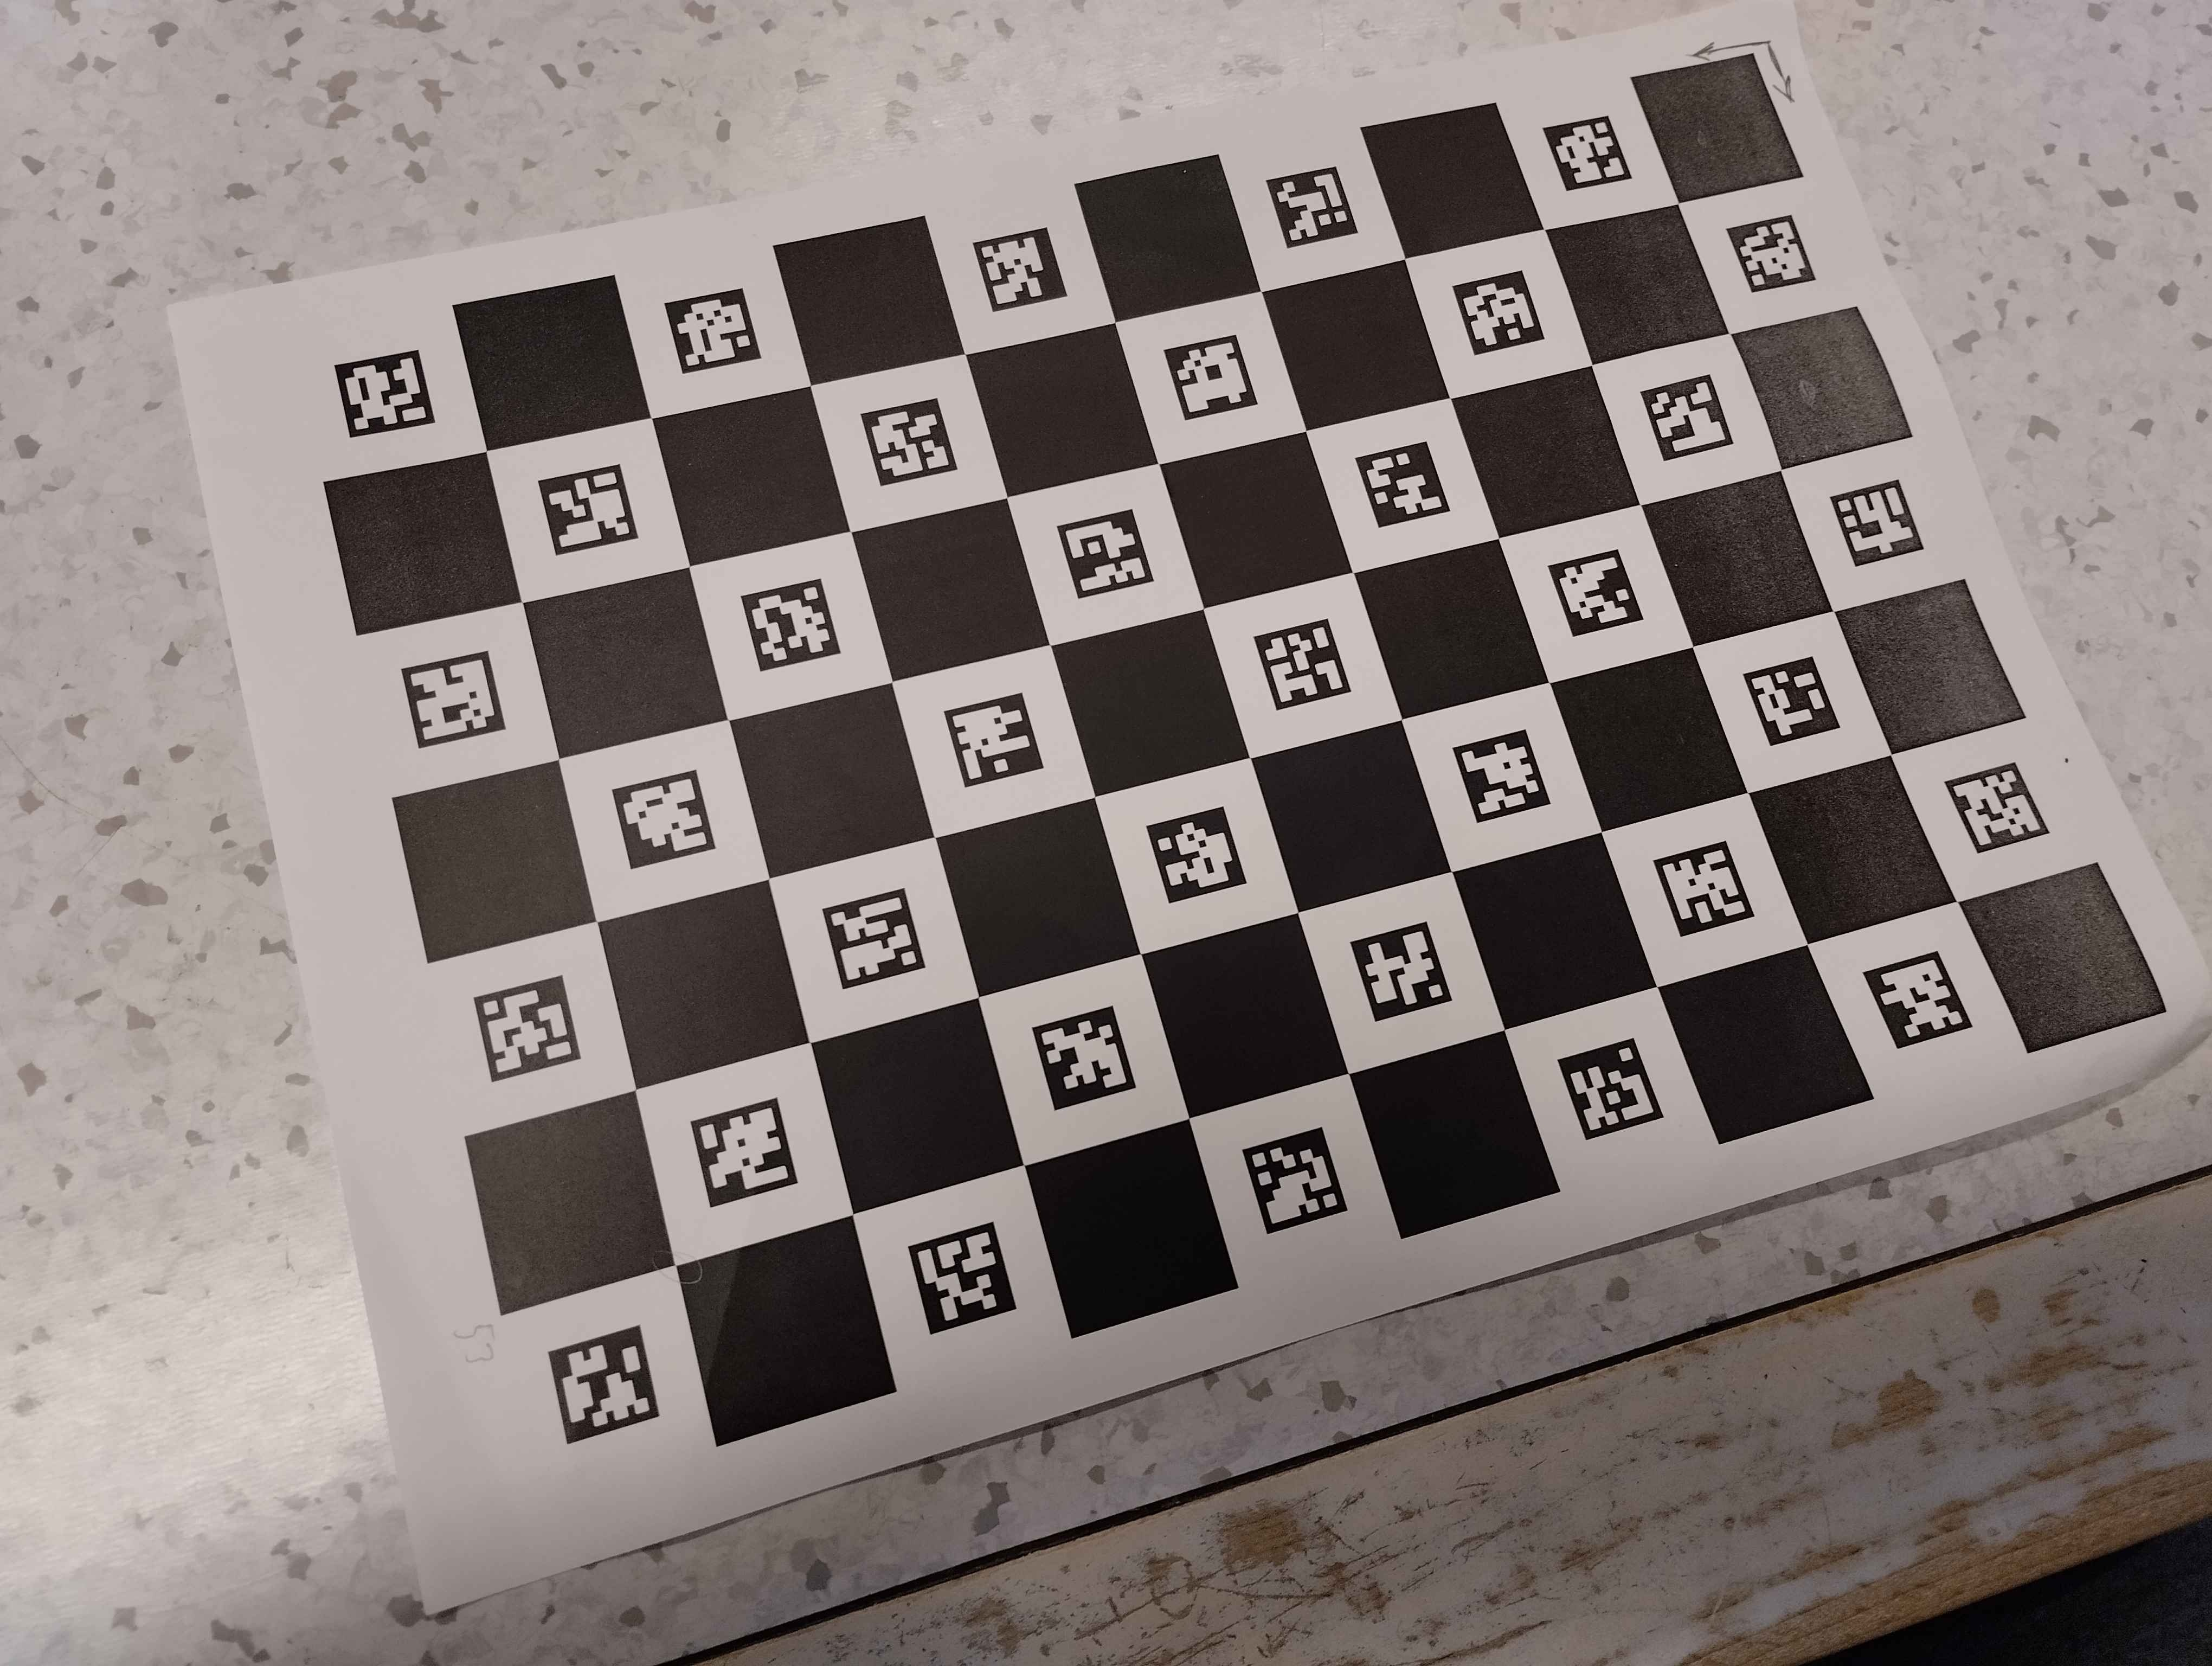
\includegraphics[width=.3\textwidth]{imgs/alphaorg.jpg}\hfill
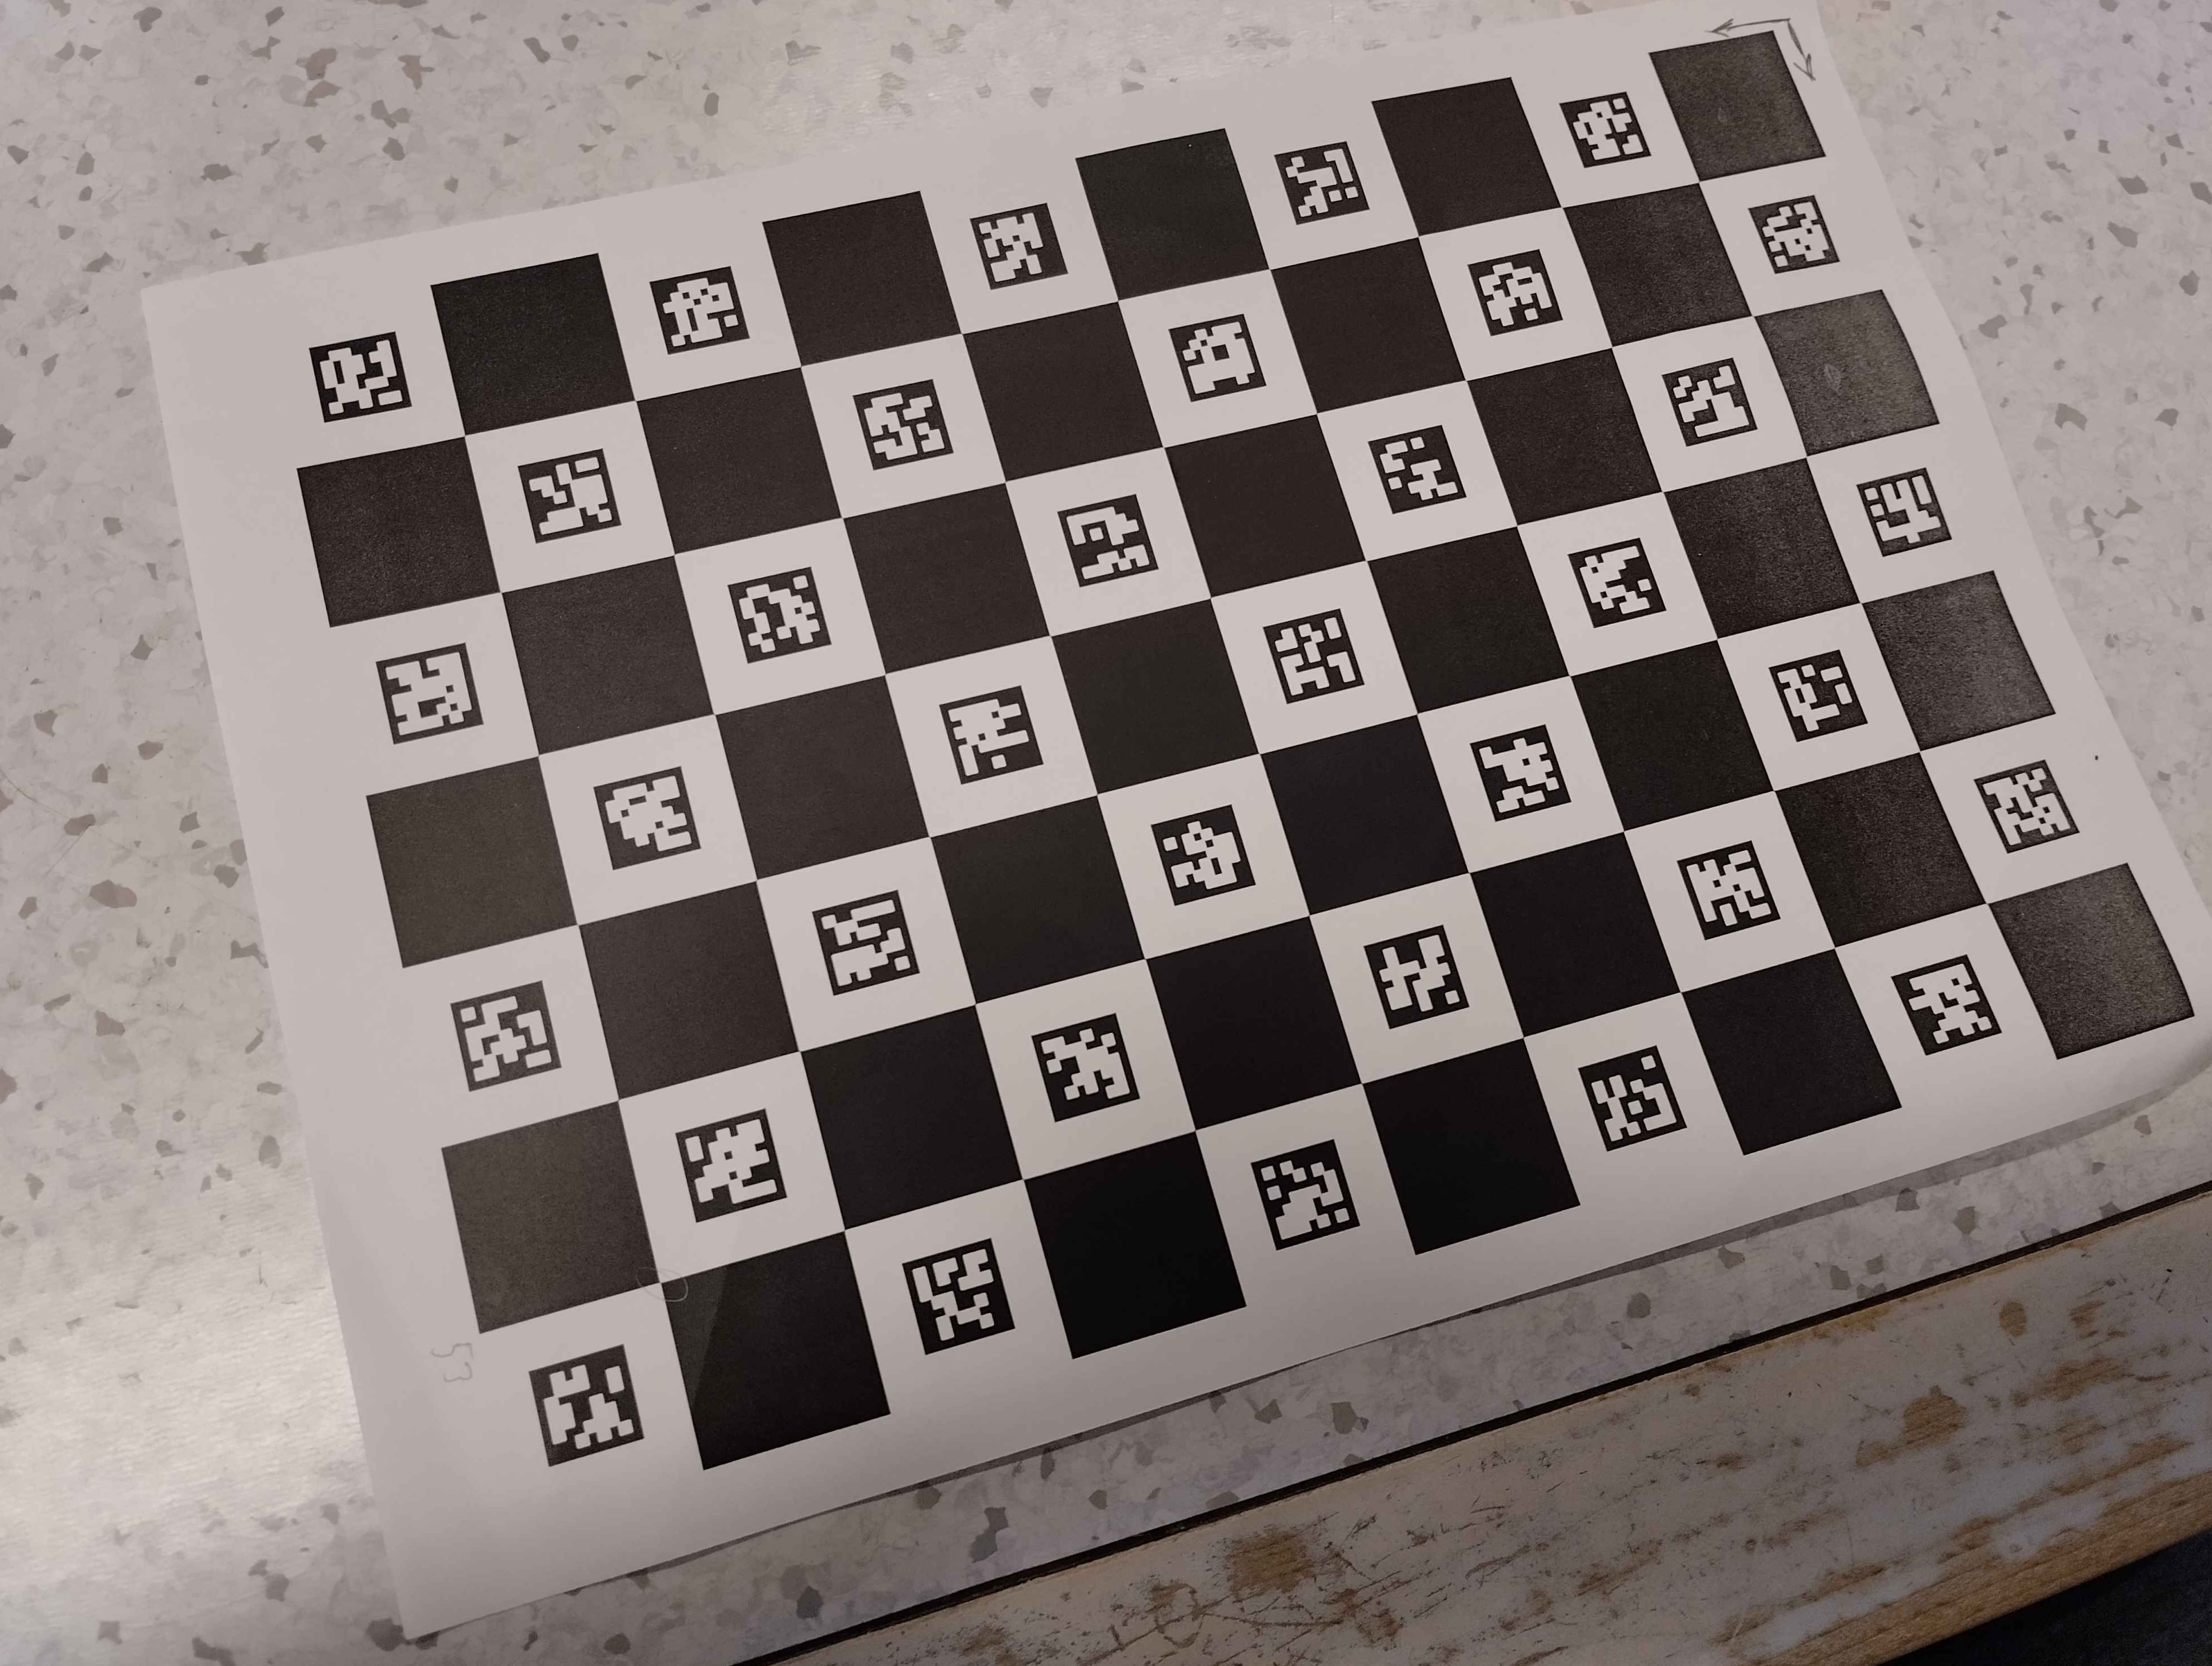
\includegraphics[width=.3\textwidth]{imgs/alpha0.jpg}\hfill
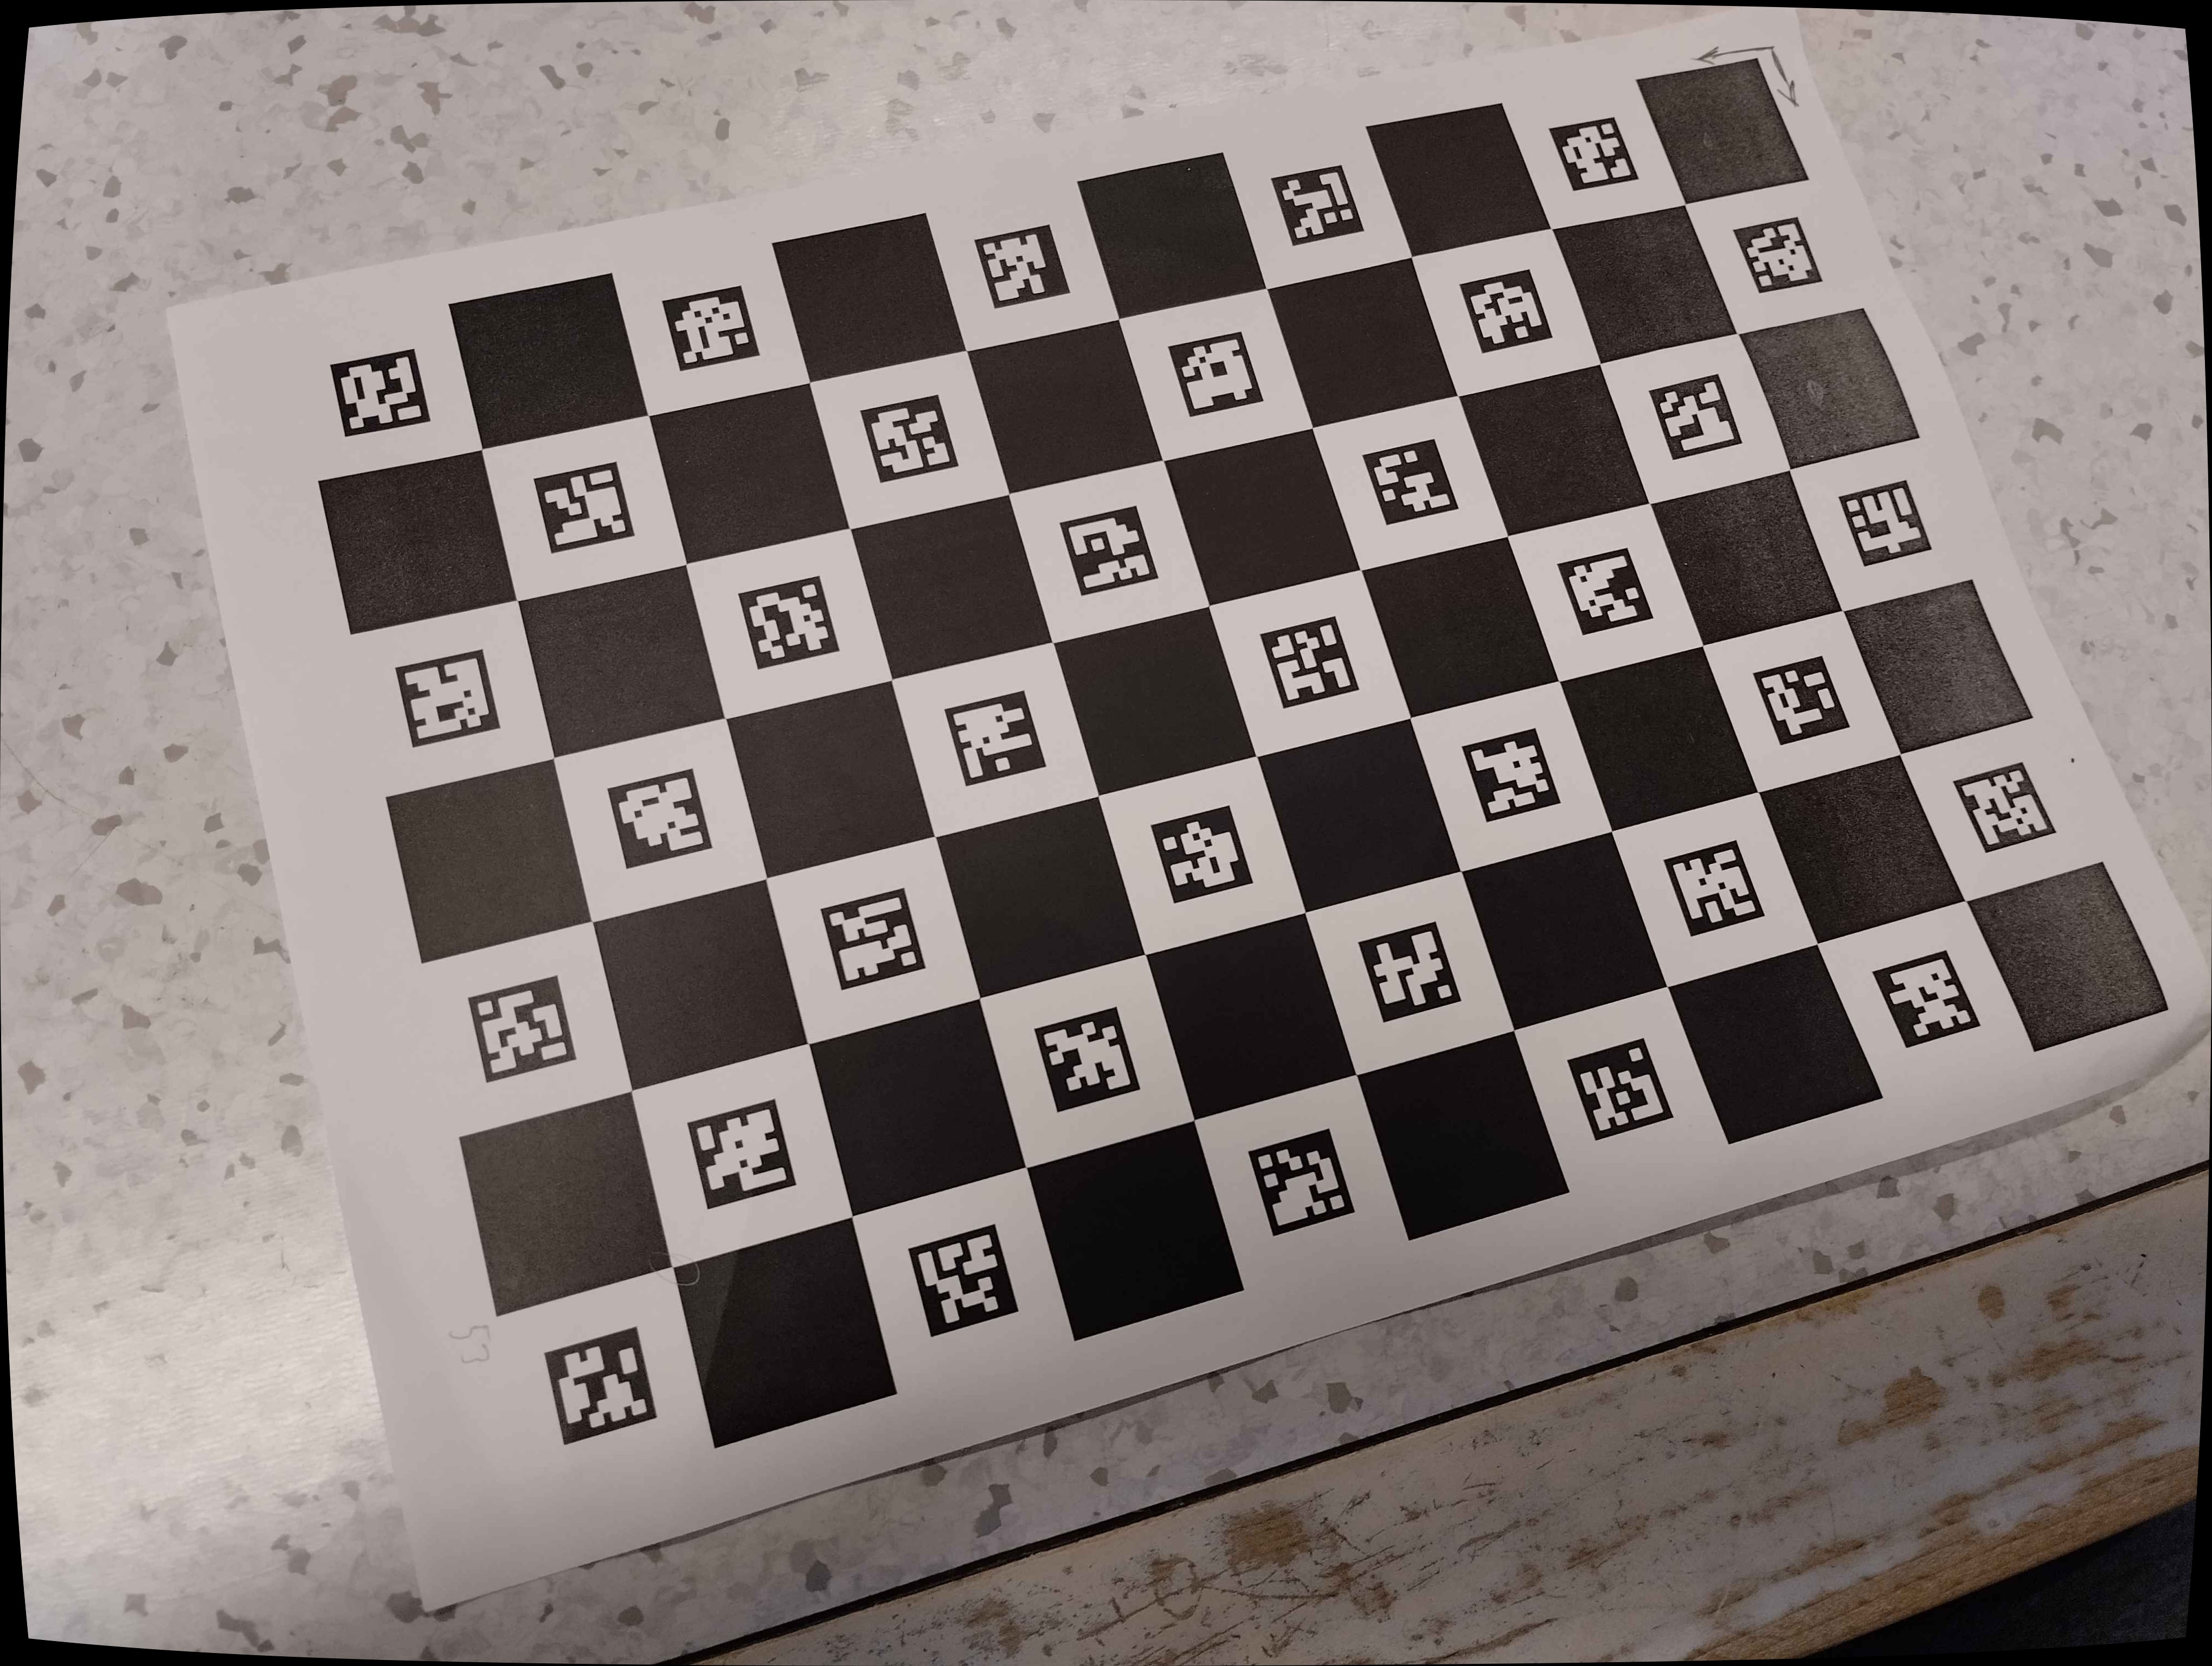
\includegraphics[width=.3\textwidth]{imgs/alpha1.jpg}

\caption{Rezultati: a) original, b) alpha=0, c) alpha=1}
\label{fig:figure3}

\end{figure}

\chapter{Meshroom}
    Meshroom je brezplačno odprtokodno orodje za 3D rekonstrukcijo, ki jo je razvilo podjetje AliceVision. Glavni način uporabe je povezovanje vozlišč, ki računajo podatke. Za začetek odprite Meshroom, izberite File$\rightarrow$New Pipeline$\rightarrow$Photogrammetry, povlecite in spustite slike predmeta, ki ga želite rekonstruirati, v galerijo slik in pritisnite Start. Ko vozlišča končajo z računanjem, jih lahko dvakrat kliknete, da si ogledate njihove rezultate. \cite{Meshroom}

\section{Vozlišča}

\subsection{CameraInit}
    To vozlišče obdela dane slike v podatke, ki jih Meshroom lahko uporabi. Prav tako bere metadata s slik, da pridobi informacije, ki jih je mogoče pozneje uporabiti v cevovodu, na primer goriščno razdaljo ali notranje parametre kamere.


\subsection{FeatureExtraction}
    To vozlišče iz slik izvleče različne točke, imenovane ``features". V njegovih parametrih lahko določimo, katero metodo lahko uporabimo. Privzeta in velikokrat najboljša metoda je dspsift (domain size pooling scale invariant feature transform), vendar obstaja tudi metoda akaze, ki se lahko uporablja za zahtevne površine, kot je koža. Tukaj lahko določimo tudi ekstrahiranje točk s cctags, ki jih lahko uporabimo za skaliranje končnega modela, tako da določimo položaje teh oznak v resničnem svetu (Opomba: če uporabljate cctags, mora imeti vsaka slika vsaj 1 viden cctag in slike je treba zmanjšati na približno 1920x1080, ker ima trdo kodirano omejitev MAX\_RESOLUTION).
    V nastavitvah tega vozlišča lahko podamo tudi maske za slike, tako da ekstrahira samo točke v danem polju na sliki. Prav tako lahko spremenimo količino in kakovost pridobljenih točk.
    
\subsection{ImageMatching}
    To vozlišče se ujema s slikami, tako da vemo, katere slike so blizu, da jih lahko pozneje uporabimo za FeatureMatching. Obstaja več metod ImageMatching. VocabularyTree razvršča in primerja ekstrahirane lastnosti vsake slike. Sequential ujema slike na podlagi njihovega imena. Exhaustive ujema vsako sliko z vsako sliko. Frustum ujema na podlagi znanih poz in ujema slike v bližini.

\subsection{FeatureMatching}
    To vozlišče pregleda najdene pare slik in najde podobne lastnosti na obeh slikah. V nastavitvah je parameter, imenovan minimal 2D motion. Privzeto je -1, kar pomeni onemogočeno, če pa ga postavimo na neko pozitivno vrednost, na primer 2, določimo, da se točka, ki naj se ujema, ne sme biti v istem položaju na obeh slikah. Ta možnost je uporabna za filtriranje ujemanj v ozadju, če uporabljamo vrtljive mize, ker je ozadje statično.

\subsection{StructureFromMotion}
    To vozlišče uporablja ta ujemanja in te podatke uporablja za prikaz položaja teh točk v 3D-prostoru ter poze (položaj in orientacija) in notranje kalibracije vseh kamer.

\subsection{PrepareDenseScene}
    To vozlišče nepopači slike. Za izračun nepopačenih slik uporablja kalibracijske parametre iz StructureFromMotion.

\subsection{DepthMap and DepthMapFilter}
    Ta vozlišča izračunajo globino slik. Filter izloči nekoherentne vrednosti globine. Določimo lahko faktor znižanje, nižji kot je faktor, večja je kakovost, a daljši je čas izračuna. 1 bi morali uporabiti samo, če imamo zelo kakovostne slike.

\subsection{Meshing and MeshFiltering}
    Mreže se izvajajo iz podatkov SfM in globin. Rezultat je gosta geometrijska površinska predstavitev scene. To mrežo lahko nato uporabimo laplaciansko filtriranje, da odstranimo lokalne napake. V nastavitvah lahko določimo vrsto izhodne datoteke, ki jo najdemo v mapi MeshroomCache, in jo lahko odpremo in manipuliramo z drugimi aplikacijami, kot je Blender.

\subsection{Texturing}
    To vozlišče teksturira mrežo. Za vsak trikotnik uporabi informacije o vidnosti, povezane z vsakim vozliščem, da pridobi kandidate za teksturo. Izbere najboljše kamere glede na ločljivost, ki pokriva trikotnik. Končno izračuna povprečje vrednosti slikovnih pik z uporabo več pasov v frekvenčni domeni.

\section{Post processing}
    Uporabimo lahko aplikacijo, kot je Blender, da si ogledamo in manipuliramo z mrežo rezultatov. Najpogosteje lahko izrežemo neželene dele iz naše mreže, skaliramo mrežo na podlagi znane geometrije in nato opravimo meritve rekonstruiranega objekta.

\section{Rezultati}
    Da bi prikazali funkcionalnost Meshrooma, bomo analizirali naslednje rekonstrukcije, ki sem jih naredil in jih naknadno obdelal v Blenderju.

    \subsection{Kitara}
    Ta model je bil narejen iz 310 slik iz različnih kotov. Kitara je bila postavljena na sredino mize, miza pa med 2 stropni svetilki, tako da je osvetlitev večinoma enaka z obeh strani. Slike so bile posnete s telefonom, ki sem ga držal. Ker sem ga držal in moja roka ni zelo stabilna, sem moral uporabiti nizka hitrost zaklopa, 1/25 s na teh slikah, zaradi česar so bile slike temne, in v nasprotju s tem sem uporabil visok ISO faktor 1200. Na mizo sem postavil tudi CCTags, vendar mi je Meshroom povzročal težave pri skaliranju, kar bom v prihodnosti popravil, in jih uporabil v Blenderju za skaliranje modela. Iz rezultatov lahko vidimo, da je bil velik del moje sobe rekonstruiran iz ozadja slik, čeprav ne preveč podrobno. Ena od stvari, ki jih Meshroom uporablja za ujemanje, so tudi podrobnosti ozadja, kar je v tem primeru super, ker je vsak kot ozadja edinstven. Kitaro sem izrezal iz modela v Blenderju. Vidimo lahko, da so vrat kitare in nesijajni deli zelo dobro rekonstruirani. Največja napaka je v trupu kitare. Tam, kjer je kitara najbolj sijoča, je velika luknja, to je zaradi odseva svetilk na trupu kitare. V prihodnosti se to lahko odstrani z uporabo polarizacijskega filtra, z mat barvo na predmetu ali z boljšo osvetlitvijo. Tudi slike za ta model so bile posnete v formatu JPG in RAW. Rezultati rekonstrukcije so pokazali, da so JPG slike veliko boljše od tistih v RAW formatu.
    
        \begin{figure}[h]
            \begin{subfigure}{.5\textwidth}
                \centering
                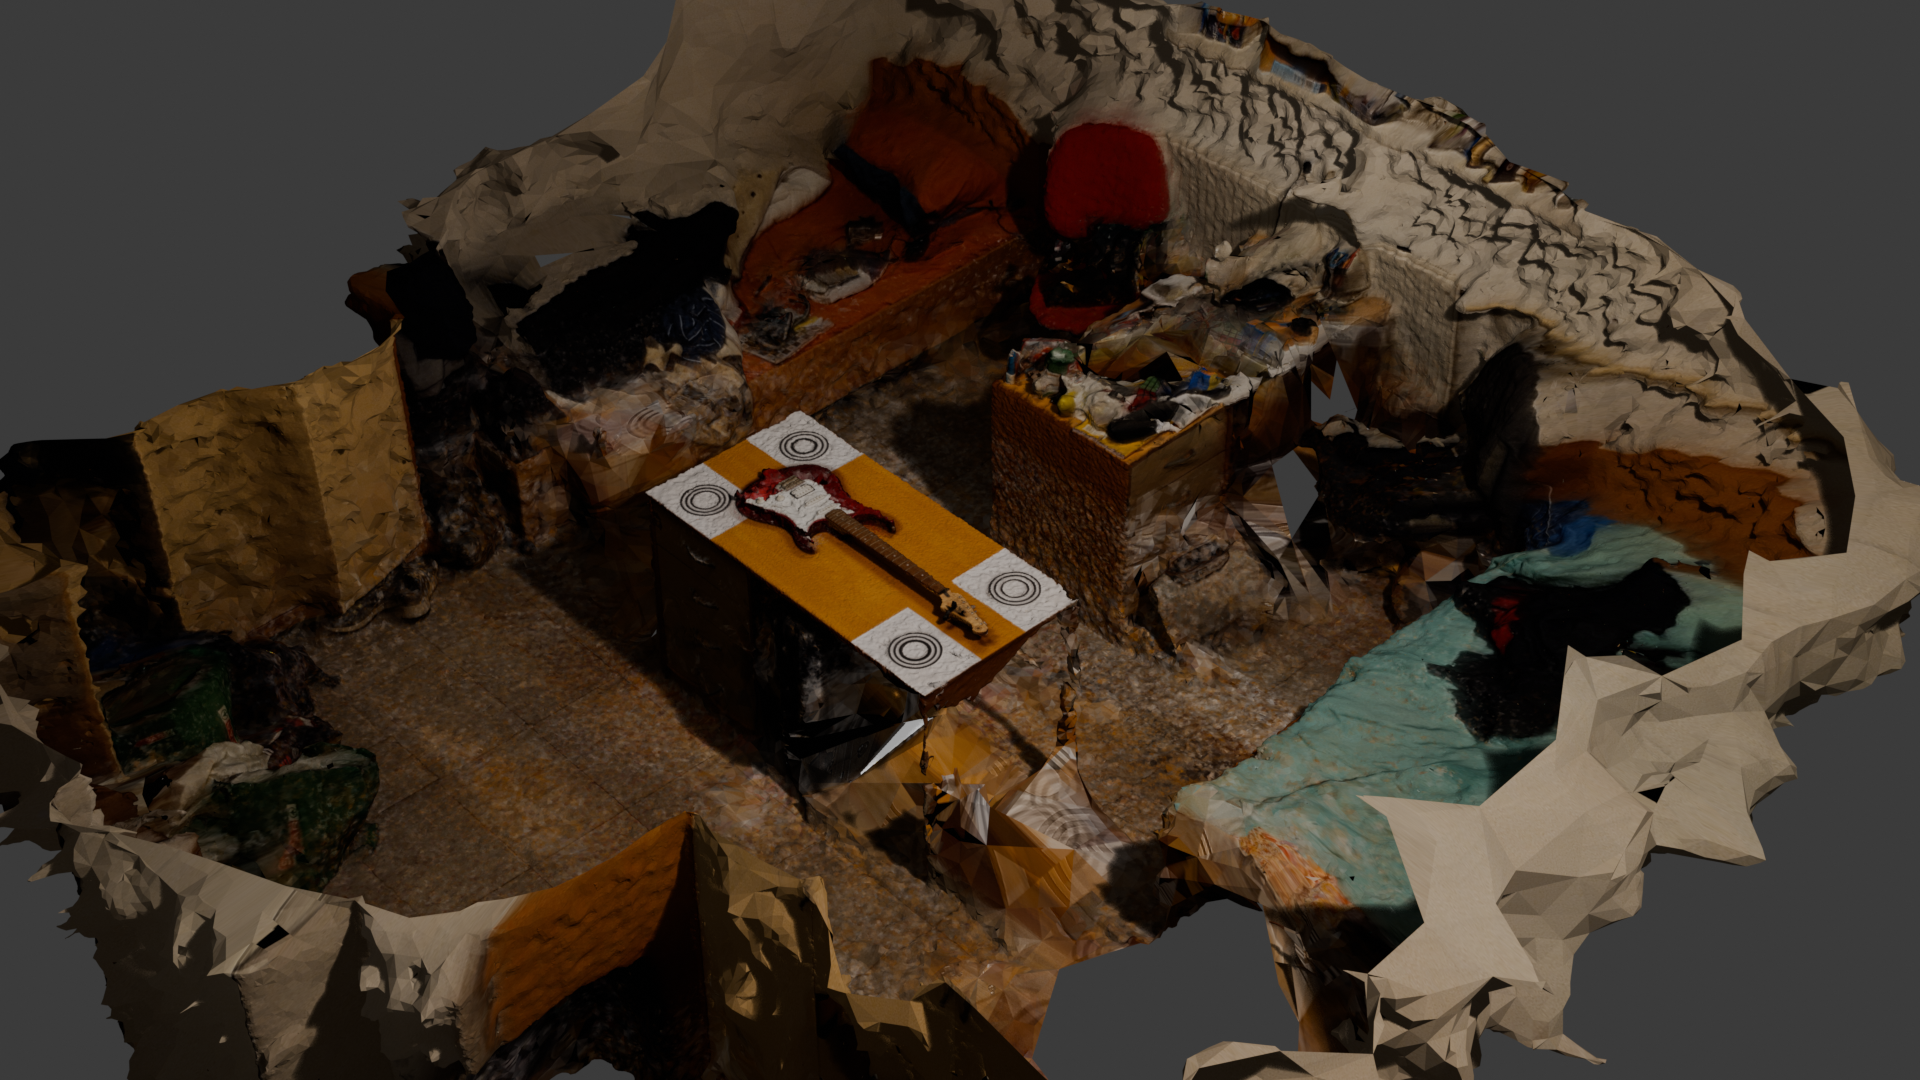
\includegraphics[width=.95\linewidth]{imgs/guitarsoba.png}
                \caption{Celoten rezultat iz Meshrooma}
            \end{subfigure}
            \begin{subfigure}{.5\textwidth}
                \centering
                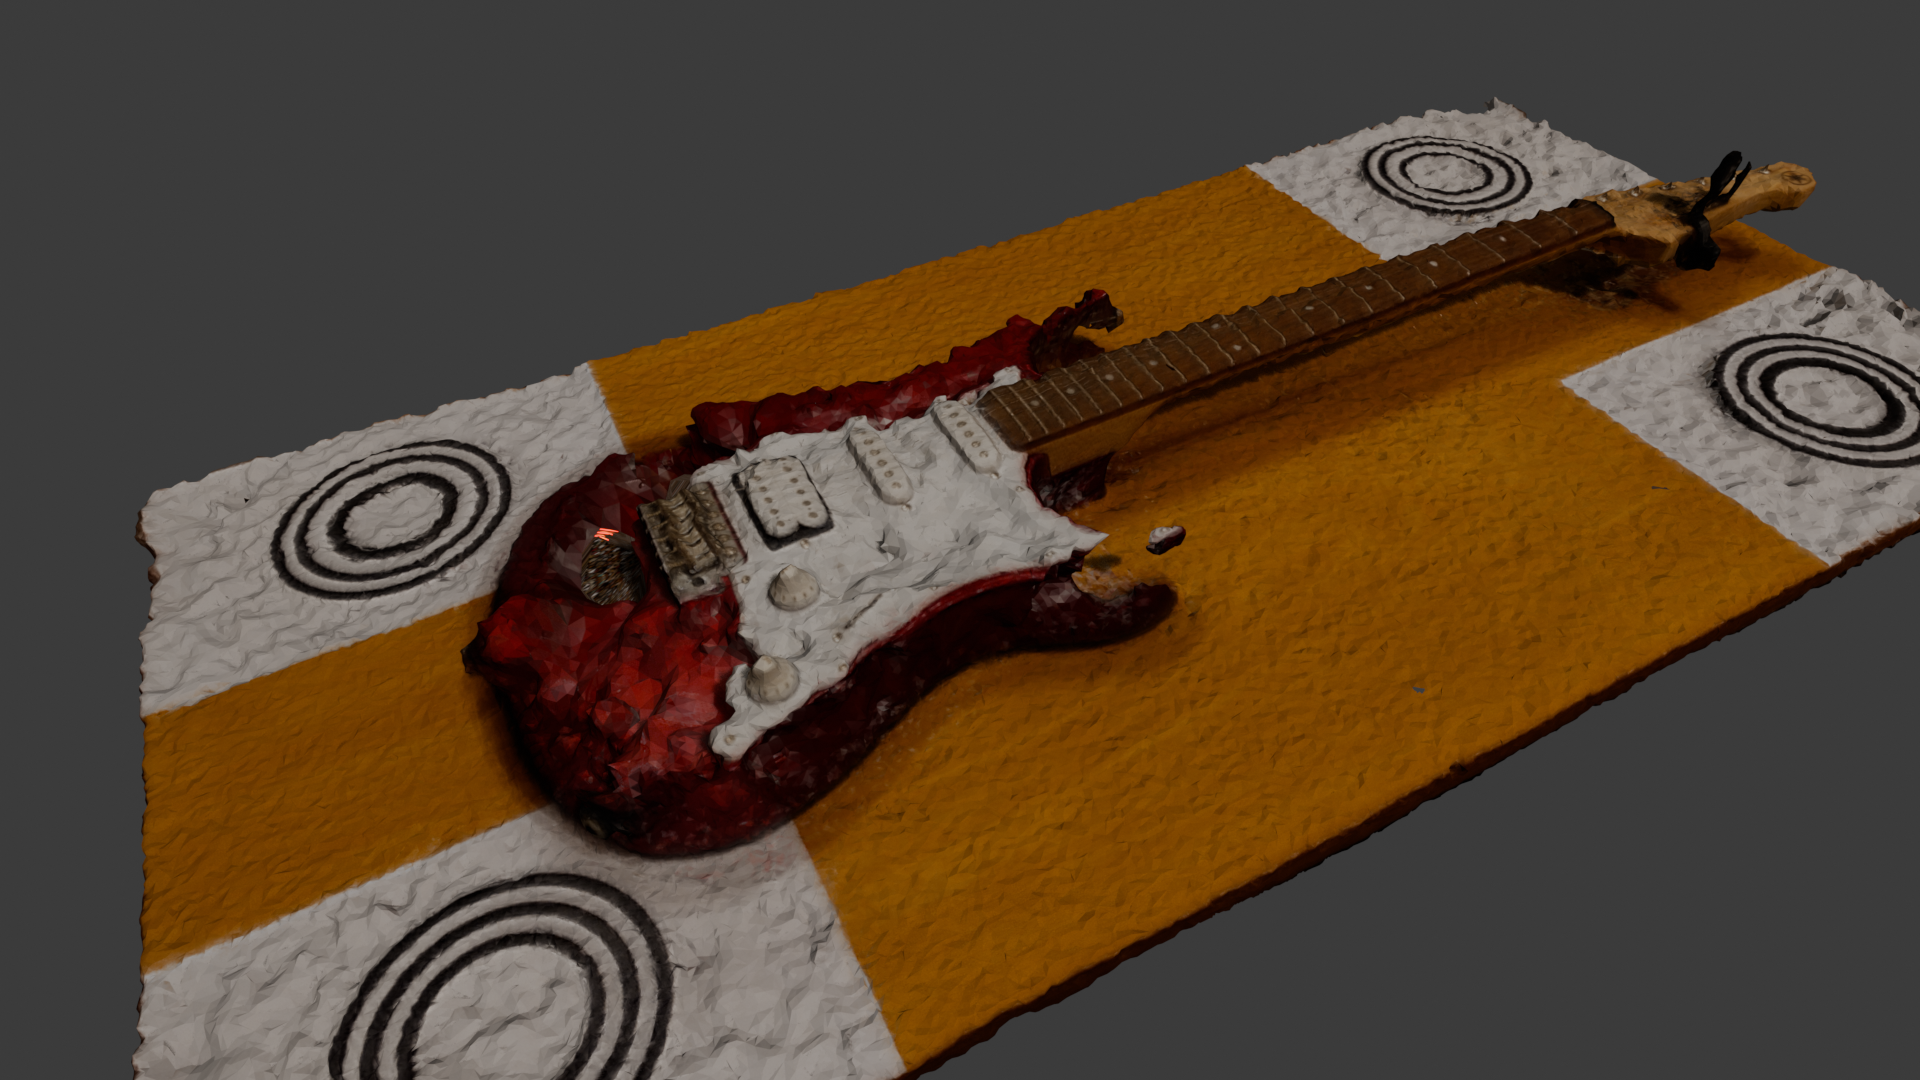
\includegraphics[width=.95\linewidth]{imgs/guitarcut.png}
                \caption{Izrezan rezultat}
            \end{subfigure}
            \caption{Rekonstrukcija kitare}
        \end{figure}
    
    \subsection{Veka}
        Ta model je bil narejen iz 34 slik moje modrice od blizu. Ideja je bila preizkusiti, koliko podrobnosti je mogoče ujeti na obrazu in modrici. Osvetlitev je bila namizna svetilka, usmerjena proti veki. Hitrost zaklopa je 1/20 s, ISO pa 150. Slike so bile posnete z ročnim telefonom. Rekonstrukcijo sem naredil z različnimi parametri, da jih je mogoče primerjati. Statistika o objektih je vidna v tabeli \ref{tab:objstat}. Vidimo lahko, da je za ta primer DSPSift veliko boljši od Akaze. Vidimo lahko tudi, da z višjimi nastavitvami dosežemo boljše rezultate, vendar je razlika med visoko in ultra zelo majhna. Iz spodnjih slik lahko opazimo, da ima Akaze veliko več ``valov" ykot DSPSift.  

        \begin{table}[h]
            \centering
            \begin{tabular}{|c|c|c|c|c|c|} \hline 
                 &  DSPSift Normal&  DSPSift High&  DSPSift Ultra&  DSPSift+Akaze& Akaze\\ \hline 
                 Vertices&  319630&  325135&  325175&  324528& 151640\\ \hline 
                 Edges&  952816&  968875&  969452&  967321& 451475\\ \hline 
                 Faces&  635128&  645823&  646201&  644784& 300898\\ \hline
            \end{tabular}
            \caption{Statistika objektov}
            \label{tab:objstat}
        \end{table}

        \begin{figure}[h]
            \begin{subfigure}{.5\textwidth}
                \centering
                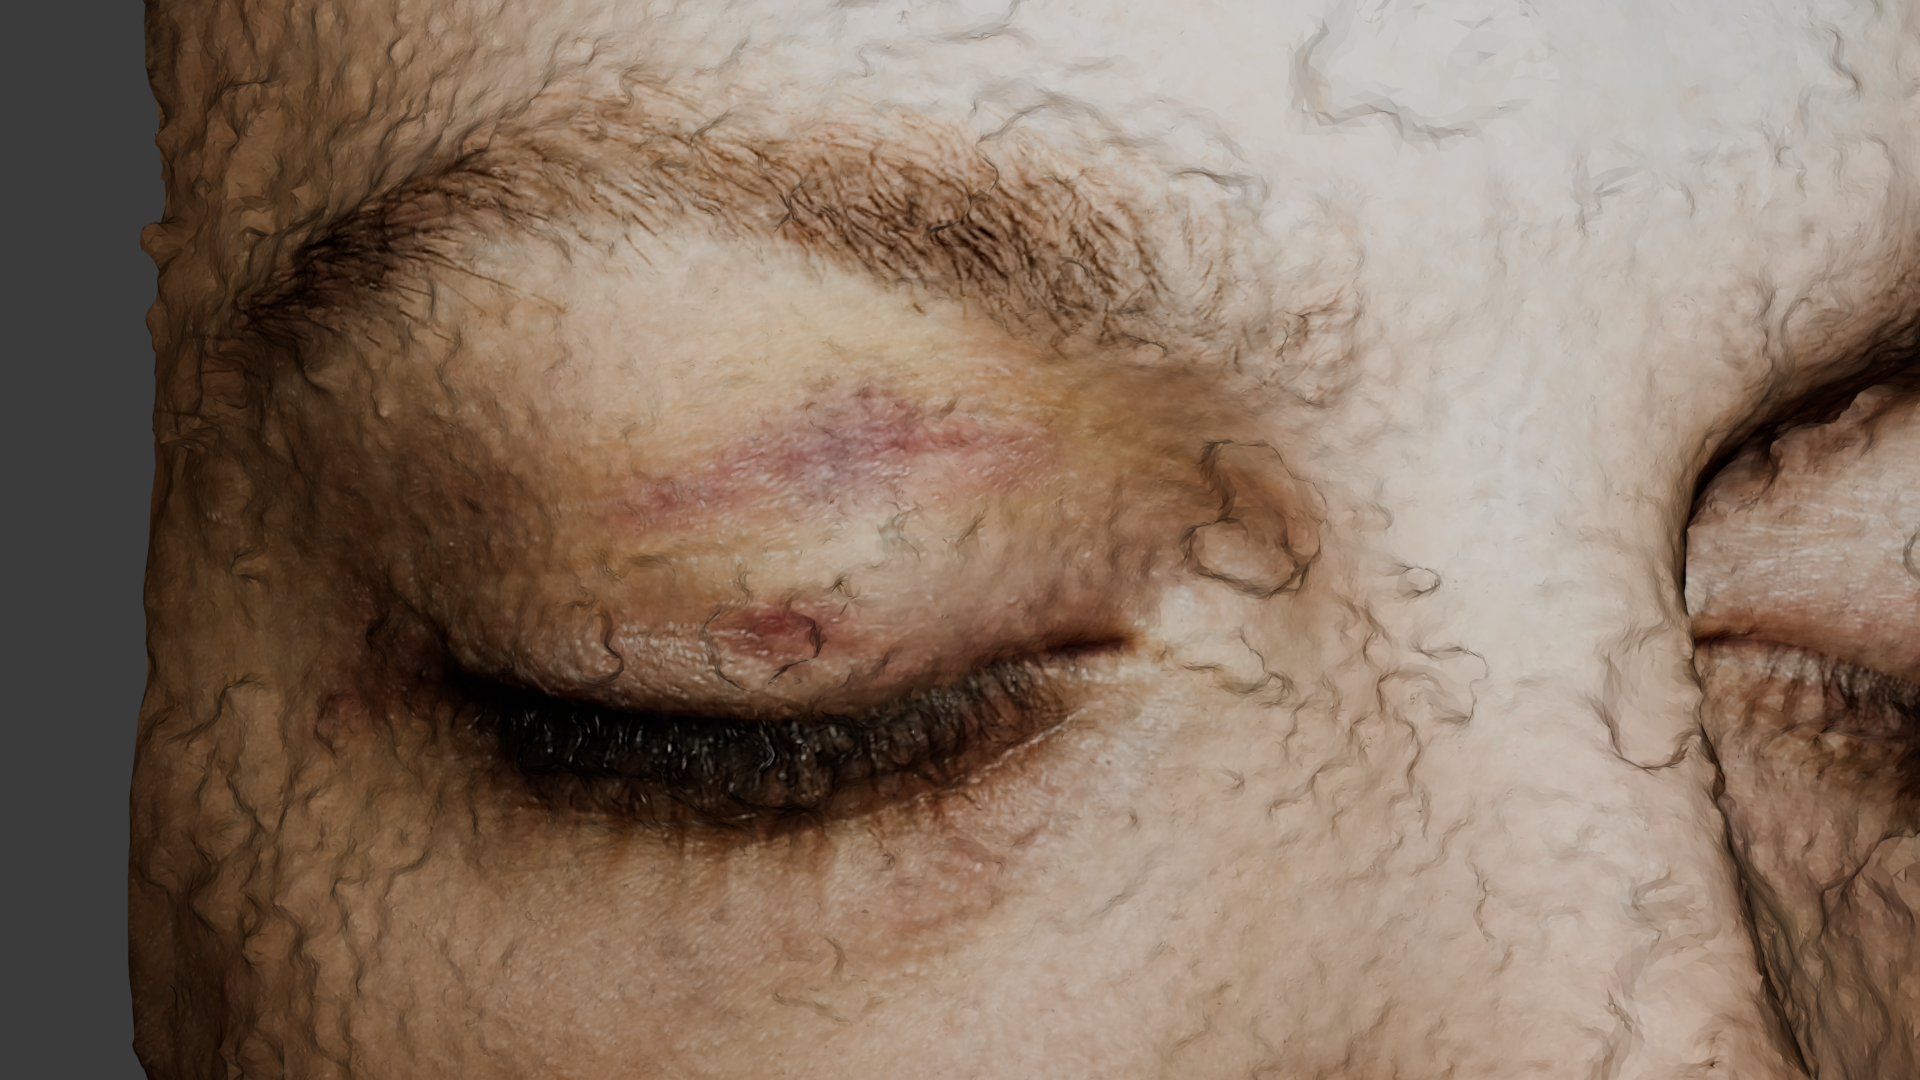
\includegraphics[width=.95\linewidth]{imgs/akaze.png}
                \caption{Akaze metoda}
            \end{subfigure}
            \begin{subfigure}{.5\textwidth}
                \centering
                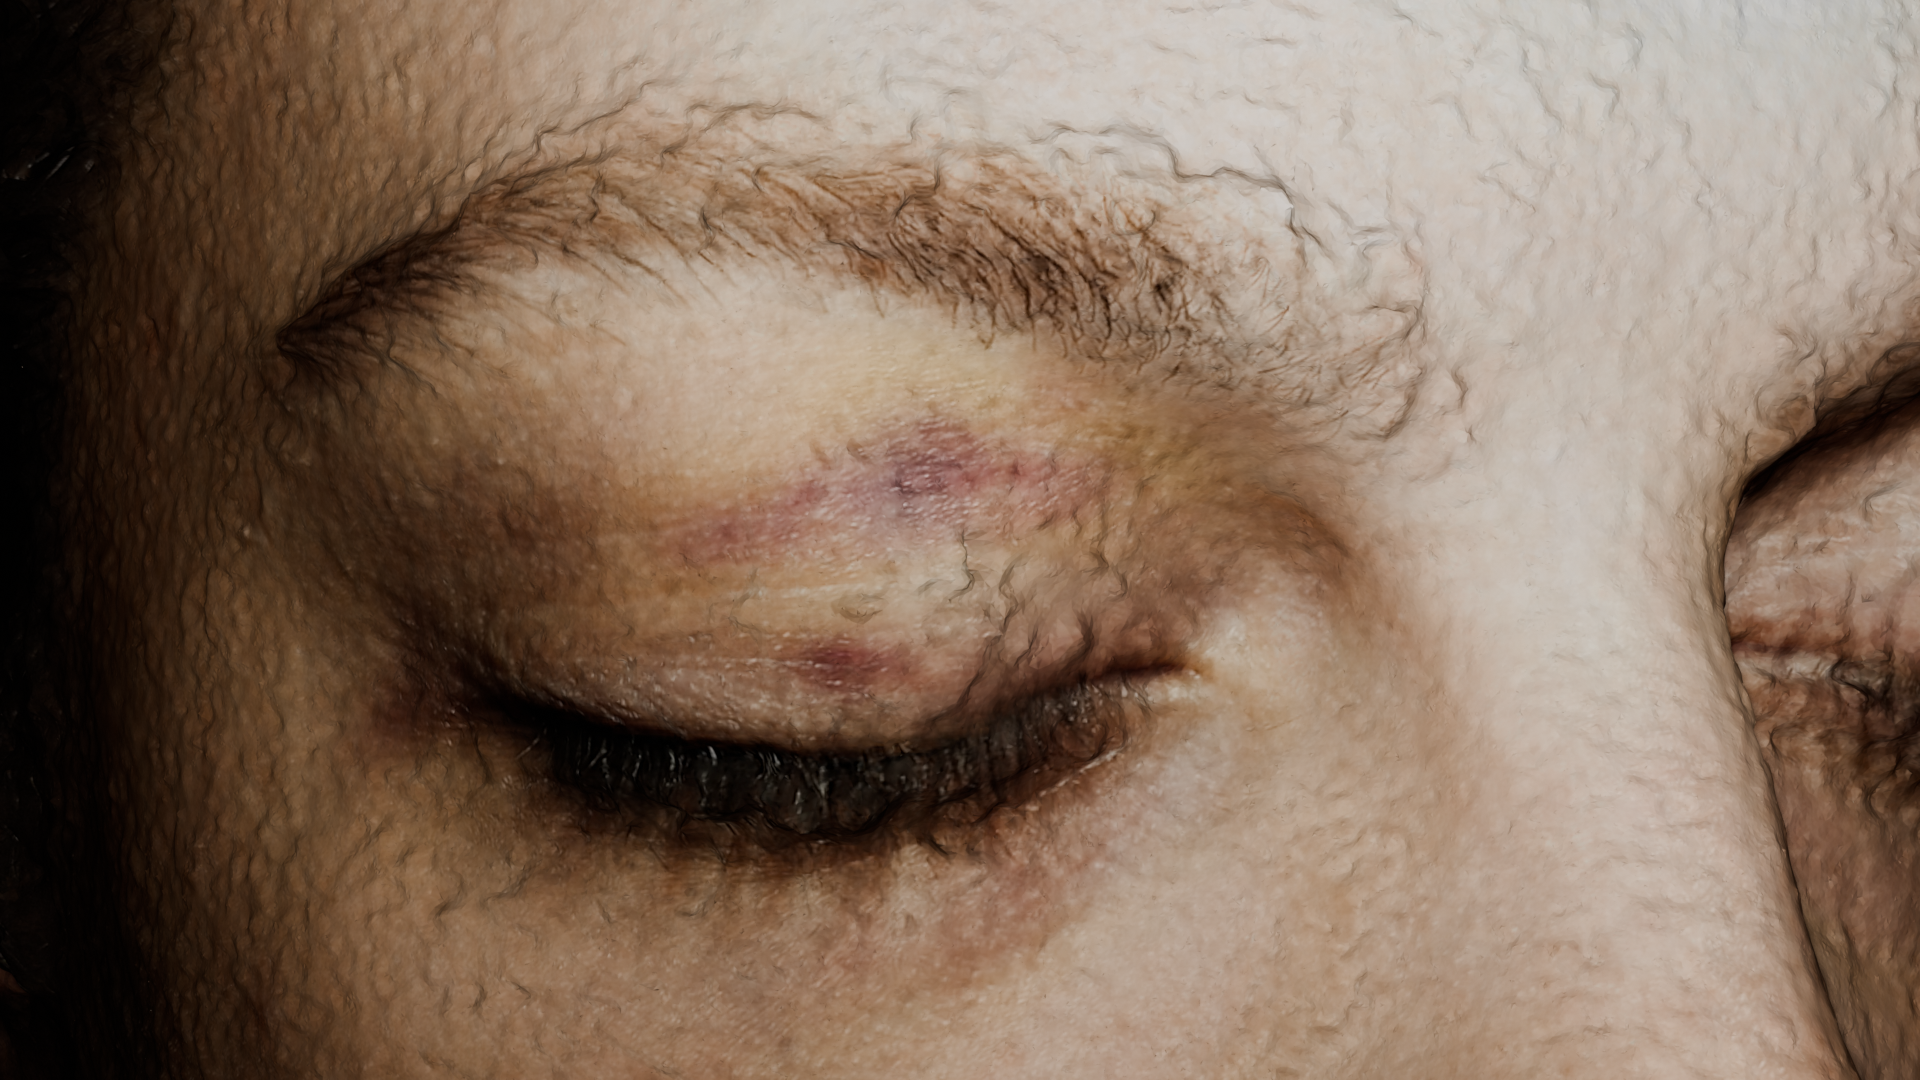
\includegraphics[width=.95\linewidth]{imgs/ultrarender.png}
                \caption{Ultra nastavitve}
            \end{subfigure}
            \caption{Rekonstrukcija vek}
        \end{figure}
    
    % \subsection{} %probaj parfem popravi ili arhitekt

    \subsection{Povzetek}
        Za dobro rekonstrukcijo moramo narediti dobre slike. Idealno bi bilo, da bi naš fotoaparat imel nižjo hitrost zaklopa in faktor ISO. Prav tako bi morali slikati v formatu JPEG in ne v formatu RAW. Osvetlitev je zelo pomembna. Moral bi biti neposredno na predmetu, ne sme ustvarjati senc. Zunanji objekt ne sme biti odseven, ker odboji svetlobnega vira povzročajo napake v rekonstruiranem modelu. Metoda DSPSift za ekstrakcijo funkcij je v preizkušenih primerih boljša od Akaze, morda pa bi bil Akaze primeren za težje površine. Nastavitve kakovosti in količine ekstrahiranih ``features" je treba spremeniti tudi glede na število slik in želeno raven podrobnosti.

% \printbibliography
\bibliographystyle{IEEEtran_slo}
\renewcommand{\thechapter}{}
\bibliography{refs}

\end{document}
